
%%%%%%%%%%%%%%%%%%%%%%%%%%%%%%%%%%%%%%%%%%%%%%%%%%%%%%%%%%%%%%%%%%%%%
%% This is a (brief) model paper using the achemso class
%% The document class accepts keyval options, which should include
%% the target journal and optionally the manuscript type.
%%%%%%%%%%%%%%%%%%%%%%%%%%%%%%%%%%%%%%%%%%%%%%%%%%%%%%%%%%%%%%%%%%%%%
\documentclass[journal=apchd5,manuscript=article]{achemso}

%%%%%%%%%%%%%%%%%%%%%%%%%%%%%%%%%%%%%%%%%%%%%%%%%%%%%%%%%%%%%%%%%%%%%
%% Place any additional packages needed here.  Only include packages
%% which are essential, to avoid problems later. Do NOT use any
%% packages which require e-TeX (for example etoolbox): the e-TeX
%% extensions are not currently available on the ACS conversion
%% servers.
%%%%%%%%%%%%%%%%%%%%%%%%%%%%%%%%%%%%%%%%%%%%%%%%%%%%%%%%%%%%%%%%%%%%%
\usepackage[version=3]{mhchem} % Formula subscripts using \ce{}
\usepackage[T1]{fontenc}       % Use modern font encodings
\usepackage{graphicx}
\usepackage{amsmath}
\usepackage{xcolor}
\usepackage{wrapfig}
%%%%%%%%%%%%%%%%%%%%%%%%%%%%%%%%%%%%%%%%%%%%%%%%%%%%%%%%%%%%%%%%%%%%%
%% If issues arise when submitting your manuscript, you may want to
%% un-comment the next line.  This provides information on the
%% version of every file you have used.
%%%%%%%%%%%%%%%%%%%%%%%%%%%%%%%%%%%%%%%%%%%%%%%%%%%%%%%%%%%%%%%%%%%%%
%%\listfiles

%%%%%%%%%%%%%%%%%%%%%%%%%%%%%%%%%%%%%%%%%%%%%%%%%%%%%%%%%%%%%%%%%%%%%
%% Place any additional macros here.  Please use \newcommand* where
%% possible, and avoid layout-changing macros (which are not used
%% when typesetting).
%%%%%%%%%%%%%%%%%%%%%%%%%%%%%%%%%%%%%%%%%%%%%%%%%%%%%%%%%%%%%%%%%%%%%
\newcommand*\mycommand[1]{\texttt{\emph{#1}}}

%%%%%%%%%%%%%%%%%%%%%%%%%%%%%%%%%%%%%%%%%%%%%%%%%%%%%%%%%%%%%%%%%%%%%
%% Meta-data block
%% ---------------
%% Each author should be given as a separate \author command.
%%
%% Corresponding authors should have an e-mail given after the author
%% name as an \email command. Phone and fax numbers can be given
%% using \phone and \fax, respectively; this information is optional.
%%
%% The affiliation of authors is given after the authors; each
%% \affiliation command applies to all preceding authors not already
%% assigned an affiliation.
%%
%% The affiliation takes an option argument for the short name.  This
%% will typically be something like "University of Somewhere".
%%
%% The \altaffiliation macro should be used for new address, etc.
%% On the other hand, \alsoaffiliation is used on a per author basis
%% when authors are associated with multiple institutions.
%%%%%%%%%%%%%%%%%%%%%%%%%%%%%%%%%%%%%%%%%%%%%%%%%%%%%%%%%%%%%%%%%%%%%
\author{Nicholas P. Montoni}
\author{Steven C. Quillin}
\author{Charles Cherqui}
\author{David J. Maisello}
\affiliation[Department of Chemistry, University of Washington]
{Department of Chemistry, University of Washington, Seattle, WA 98195}
\email{masiello@chem.washington.edu}
\date{September 4, 2017}
%%%%%%%%%%%%%%%%%%%%%%%%%%%%%%%%%%%%%%%%%%%%%%%%%%%%%%%%%%%%%%%%%%%%%
%% The document title should be given as usual. Some journals require
%% a running title from the author: this should be supplied as an
%% optional argument to \title.
%%%%%%%%%%%%%%%%%%%%%%%%%%%%%%%%%%%%%%%%%%%%%%%%%%%%%%%%%%%%%%%%%%%%%
\title[]
    {Tunable Spectral Ordering and Directional Radiation in Magnetic Plasmon Oligomers}
%%%%%%%%%%%%%%%%%%%%%%%%%%%%%%%%%%%%%%%%%%%%%%%%%%%%%%%%%%%%%%%%%%%%%
%% Some journals require a list of abbreviations or keywords to be
%% supplied. These should be set up here, and will be printed after
%% the title and author information, if needed.
%%%%%%%%%%%%%%%%%%%%%%%%%%%%%%%%%%%%%%%%%%%%%%%%%%%%%%%%%%%%%%%%%%%%%
\abbreviations{MNP, LSPR, EELS}
\keywords{plasmon, hybridization, magnetic, retardation}

%%%%%%%%%%%%%%%%%%%%%%%%%%%%%%%%%%%%%%%%%%%%%%%%%%%%%%%%%%%%%%%%%%%%%
%% The manuscript does not need to include \maketitle, which is
%% executed automatically.
%%%%%%%%%%%%%%%%%%%%%%%%%%%%%%%%%%%%%%%%%%%%%%%%%%%%%%%%%%%%%%%%%%%%%
\begin{document}

%%%%%%%%%%%%%%%%%%%%%%%%%%%%%%%%%%%%%%%%%%%%%%%%%%%%%%%%%%%%%%%%%%%%%
%% The "tocentry" environment can be used to create an entry for the
%% graphical table of contents. It is given here as some journals
%% require that it is printed as part of the abstract page. It will
%% be automatically moved as appropriate.
%%%%%%%%%%%%%%%%%%%%%%%%%%%%%%%%%%%%%%%%%%%%%%%%%%%%%%%%%%%%%%%%%%%%%
\begin{tocentry}

Some journals require a graphical entry for the Table of Contents.
This should be laid out ``print ready'' so that the sizing of the
text is correct.

Inside the \texttt{tocentry} environment, the font used is Helvetica
8\,pt, as required by \emph{Journal of the American Chemical
Society}.

The surrounding frame is 9\,cm by 3.5\,cm, which is the maximum
permitted for  \emph{Journal of the American Chemical Society}
graphical table of content entries. The box will not resize if the
content is too big: instead it will overflow the edge of the box.

This box and the associated title will always be printed on a
separate page at the end of the document.

\end{tocentry}

%%%%%%%%%%%%%%%%%%%%%%%%%%%%%%%%%%%%%%%%%%%%%%%%%%%%%%%%%%%%%%%%%%%%%
%% The abstract environment will automatically gobble the contents
%% if an abstract is not used by the target journal.
%%%%%%%%%%%%%%%%%%%%%%%%%%%%%%%%%%%%%%%%%%%%%%%%%%%%%%%%%%%%%%%%%%%%%
\begin{abstract}
Magnetic plasmon resonances, the collective response of cyclic arrangements of plasmonic nanoparticles, have been of great recent interest due to their ability to couple to both the electric and magnetic field of light. At small sizes, these metal nanoparticle aggregates, called magnetic oligomers, satisfy the quasistatic approximation and couple weakly to the magnetic field of light. At large sizes, the magnetic and electric effects interfere with one another, resulting in size- and frequency-dependent radiative properties. This allows for tunable and controllable directionality of light scattered from these systems, opening the path to applications that require direct control over the directionality of specific colors of light.
\end{abstract}

%%%%%%%%%%%%%%%%%%%%%%%%%%%%%%%%%%%%%%%%%%%%%%%%%%%%%%%%%%%%%%%%%%%%%
%% Start the main part of the manuscript here.
%%%%%%%%%%%%%%%%%%%%%%%%%%%%%%%%%%%%%%%%%%%%%%%%%%%%%%%%%%%%%%%%%%%%%
\section{introduction}
The collective plasmon resonances of cyclic arrangements of metal nanoparticles (MNPs), called magnetic plasmon oligomers, are known to couple to and enhance both the electric and magnetic field of light [cites]. Theoretical studies of such oligomers has often focused on either single oligomers or infinite planar arrays [cites], leaving many open questions surrunding the properties of mutli-oligomer clusters in this interemdiate size regime [cites]. In fact, there is still disagreement in the field on the energy-ordering of multiple magnetic plasmons, the effect of size on their energy ordering, and the applicability of the quasistatic approximation. While much work has been done to describe MNP dimers, chains, and arrays beyond the quasistatic limit, fully retarded models combined with full-wave simulation have not been applied to magnetic plasmon oligomers. Interestingly, because these systems store energy in their magnetic fields, it is apparent that retardation effects are in fact necessary to properly describe them.

In this work, we extend the coupled dipole approximation to include retardation effects and apply it to multi-oligomer MNP clusters to determine their magnetic normal modes and eigenenergies. In doing so, we explain a previously reported discrepancy and discover that the magnetic modes change spectral order with changing system size. Comparing these results with a quasistatic model produces an approximate limit upon the applicability of static approxiamtions. Furthermore, we show using full-wave simulations that these mode crossings are observable in angle-resolved cathodoluminescence (CL) spectroscopy, electron energy loss spectroscopy (EELS) maps, and CL maps. Finally, we show that the overlapping and interfering electric and magnetic plasmons of multi-oligomer systems produce directional radiation that would not be observable with purely electric resonances. Understanding the spectral ordering and optical properties of plasmon oligomers will aid in the construction of devices for nanoscale etching, enhancement of magnetic dipole transitions in the rare earth ions, or tunable, multi-wavelength cloaking devices.

(((due to their applicability to biological sensing and imaging, electromagnetic cloaking, and information processing\cite{Zia2010trans,Noginova2008trans,Wang:13,Fan2015,Wei2015,Shvets2012,Altug2012bio,Nord2011fano,Zhang2006,NordHal2011,NordHal2012}. These collective magnetic responses occur when three or more metal nanoparticles are arranged on the vertices of a polygon, a structure known as a magnetic plasmon oligomer. The properties of single oligomers have been well-documented, as well as the properties of infinite metal nanoparticle arrays, but there are open questions regarding the behavior of few-oligomer systems.\cite{Dionne2011,Dionne2016,Weick2013,Engheta2017,Cherqui2014,Cherqui2016} Problems such as magnetic plasmon hybridization and electric-magnetic plasmon interference are still open and are the key to utilizing the unique optical properties of magnetic oligomers.

Aggregates of metal nanoparticles resembling conjugated hydrocarbon rings have been of particular interest due to their strong enhancement of magnetic fields [\textbf{cite this 2017 paper on metal clusters, also Engheta 2017}]. Because of their unique ability to couple efficiently to both electric and magnetic fields, they make an excellent model system with which to study the size-dependence of magnetic effects in metal nanoparticle oligomers. Specifically, using conjugated hydrocarbon-like aggregates, we show that the energy ordering of magnetic plasmons is tunable, a result not found using quasistatic models. Furthermore, the interference between magnetic and electric plasmons on one oligomer is shown to be size- and frequency-dependent. 

In the single-oligomer regime, the quasistatic approximation is good and describes magnetic oligomers accurately\cite{Nord2006,Dionne2016}. While retardation effects have been considered in studies of both large MNPs and infinite MNP arrays\cite{Abajo2008,Gu2010,vonPlessen2007,Rechbacher2003,Kottman2001,Schatz2003,Royer2005,Chumanov2010,Pinchuk2016}, the breakdown of the quasistatic approximation and size-dependent tunability have not been studied in magnetic oligomers. Incorporating retardation effects into a simple model, such as the tight-binding model previously utilized\cite{Cherqui2014}, is the first step to accurately modeling magnetic plasmon-supporting aggregates. When augmented with retardation effects, this model not only explains the reason why a quasistatic model and full-wave simulations should disagree, but it shows in addition that the magnetic modes of planar, few-oligomer systems exhibit dynamic and tunable energy-ordering. As suggested by previous work, single magnetic oligomers exhibit electric-magnetic interferences.\cite{Dionne2011}  Planar, multi-oligomer systems exhibit similar properties with both size- and frequency-dependence. As a result, it is possible to use magnetic oligomers to scatter light of specific colors in different directions, suggesting increased tunability and control of light.)))

\section{Model Systems and Magnetic Plasmon Resonances}

\begin{figure}
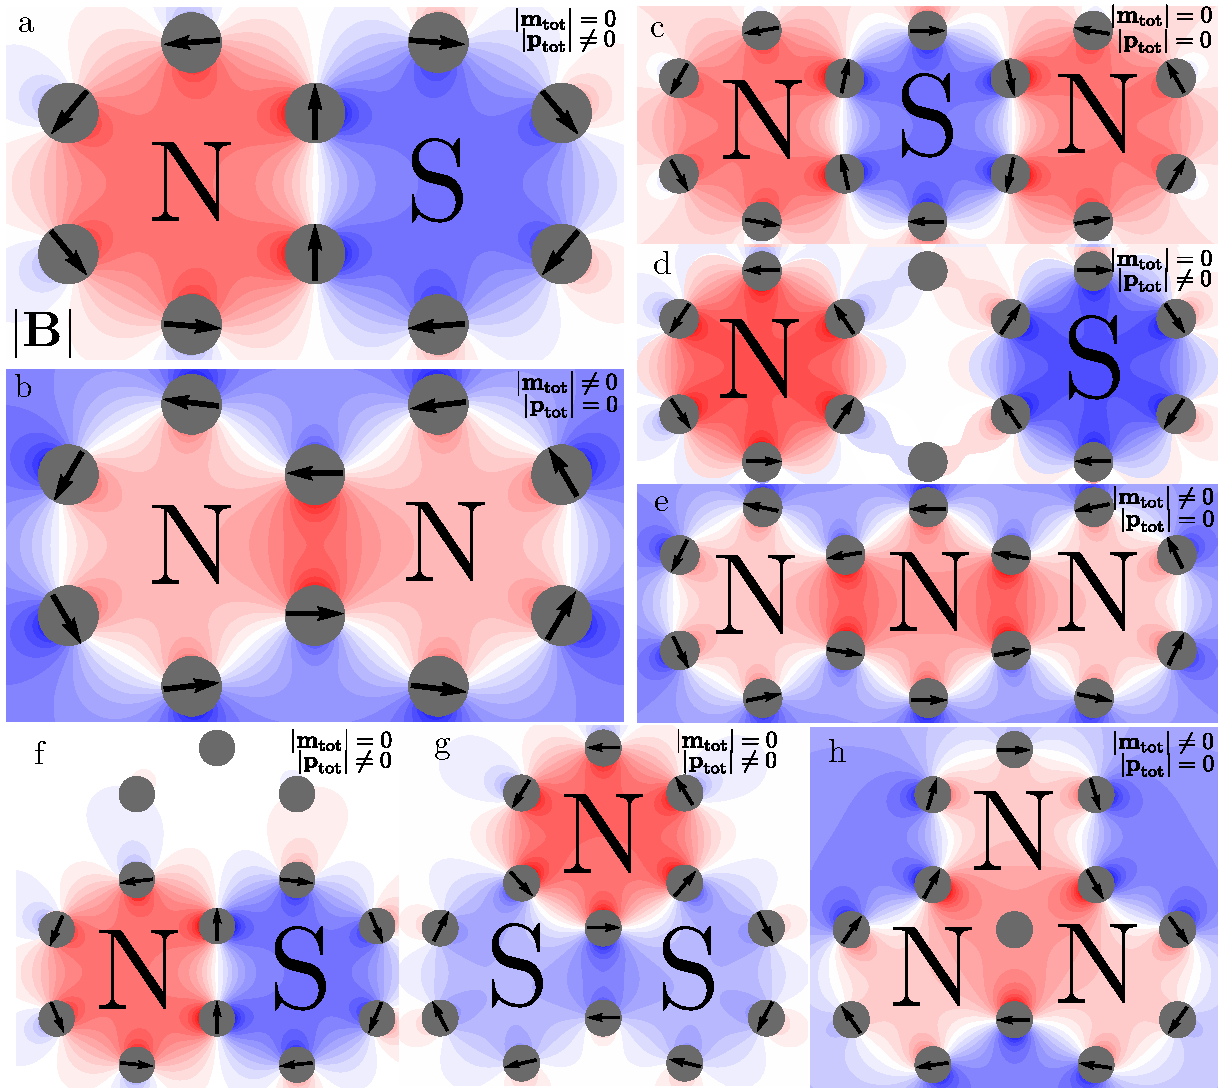
\includegraphics[width=6.5in]{fields_new_arrows.pdf}
\caption{Magnetic field plots of the two-ring (a and b), linear three-ring (c, d, and e), and triangular three-ring (f, g, and h) oligomers. Each system supports a number of closed-loop magnetic plasmon resonances equal to the number of rings in the system. The nodeless magnetic plasmons (b, e, and h) support a net magnetic dipole moment and are excitable by the magnetic field of light. The single-node magnetic plasmons (a, c, f, and g) support net electric dipole moments. The two-node magnetic mode of the linear three-ring system is inaccessible by light.}
\label{field_plots}
\end{figure}

To begin, we investigate a model system comprising two hexagonal rings fused on a side, resulting in a ten MNP aggregate resembling the molecule naphthalene. These conjugated hydrocarbon-like systems have been of great interest recently, and this system in particular represents the simplest of such systems supporting more than one magnetic plasmon. Once this system has been investigated in full, it will be extended to a more detailed system, and finally the concepts will be applied to aggregates that have been the focus of more recent research. The aggregates presented are composed of identical silver MNPs. In order to compute their collective eigenmodes and eigenenergies, we map the individual electric dipole plasmon of each MNP onto a harmonic oscillator and couple them through dipole-dipole interactions as follows\cite{ARPC}

\begin{equation}
\ddot{\textbf{q}}_i = -\omega_{\textrm{sp}}^2\textbf{q}_i + \frac{e}{m_{\textrm{sp}}}\sum_{j\neq i}\textbf{E}_j(\textbf{r}_i)
\label{equation_of_motion}
\end{equation}

\noindent where $\omega_{\textrm{sp}}$ is the natural frequency of a single electric plasmon, $m_{\textrm{sp}} = e^2/\alpha_{\textrm{sp}}\omega_{\textrm{sp}}^2$ is the surface plasmon effective mass defined by the polarizability $\alpha_{\textrm{sp}}$, the plasmon oscillator dipole moment $\textbf{d}_i = e\textbf{q}_i$, and $\textbf{E}_j(\textbf{r}_i)$ is the fully retarded electric field from the $j^{\textrm{th}}$ dipole at the position of the $i^{\textrm{th}}$ dipole and is defined as 

\begin{equation}
\textbf{E}_j(\textbf{r}_i) = \boldsymbol{\Lambda}_{ij}\cdot\textbf{d}_j\\
= \left\{\left(\frac{1}{r_{ij}^3} - \frac{ik}{r_{ij}^2}\right)\left(3\hat{\textbf{n}}_{ij}\hat{\textbf{n}}_{ij} - \textbf{1}\right) + \frac{k^2}{r_{ij}}\left(\textbf{1}-\hat{\textbf{n}}_{ij}\hat{\textbf{n}}_{ij}\right)\right\}\frac{e^{\textrm{i}kr_{ij}}}{\varepsilon_b}\cdot\textbf{d}_j.
\label{electric_field_lambda}
\end{equation}

\noindent Here, $\hat{\textbf{n}}_{ij}$ is the unit vector connecting two dipoles separated by distance $r_{ij}$, $k=\sqrt{\varepsilon_b}\omega/c$ is the wavenumber of the collective mode with frequency $\omega$, and $\varepsilon_b$ is the dielectric constant of the background medium. The fully retarded electric field contains three important terms. The term with $1/r_{ij}^3$-dependence is called the near-field, because it decays very quickly with increasing distance. In fact, this term is what remains when taking the quasistatic limit. The second term, with the $k/r_{ij}^2$-dependence, is the intermediate-field term. The third term, with $k^2/r_{ij}$-dependence, is the far-field term, called such because it dominates after the other two have decayed. All three terms are dressed by a complex exponential, which depends both on $k$ and on $r_{ij}$. This shows that at specific separation distances, the interaction energies can change sign and go from energy-lowering to energy-raising. Using just the fully retarded electric field, we have incorporated all necessary retardation effects\cite{Purcell1973}.

Solving the system of Equations~\ref{equation_of_motion} for all of the dipoles in a single aggregate yields as many hybridized modes as there are degrees of freedom, in this case, two times the number of particles. Similarly, each system supports a number of magnetic plasmons equal to the number of oligomers. The eigenvectors of these collective modes represent the dipole moments on each nanoparticle. Figure~\ref{field_plots} shows these magnetic mode eigenvectors overlayed with plots of the signed magnetic field magnitude of each normal mode. Each mode is named for its particular magnetic field distribution after the poles of a magnet (e.g. the 2-mer's North-South and North-North mode). It is important to note which magnetic modes can couple to the far-field. The top right-hand corner of each field plot in Figure~\ref{field_plots} displays whether the magnetic mode depicted exhibits a net electric dipole, a net magnetic dipole, or neither. Because it is possible to excite both a magnetic dipole moment and an electric dipole moment orthogonal to one another in these oligomers, they exhibit tunable directionality in the light that they scatter. This will be an important discussion later in this work when outlining the properties of magnetic oligomer systems. To begin, we apply the fully retarded tight-binding model to the magnetic modes of the 2mer system to determine where and why the quasistatic approximation breaks down in magnetic oligomer systems.

\section{Spectral Ordering of Magnetic Modes in the 2-mer}
To determine the breakdown of the quasistatic limit as a function of size and the impact of incorporating retardation effects, we introduce two parameters: scale and spacing. Defining a nearest-neighbor distance between individual nanoparticles $r_{\textrm{nn}} = (s + 2)r_0$ allows both scale (changing $r_0$ with fixed $s$) and spacing (changing $s$ withfixed $r_0$) to be vary independently. Figure~\ref{scaling} shows the results of varying both $r_0$ (a-d) and $s$ (e-h) in vacuum and in water ($\varepsilon_b = 1.77$). At small sizes the magnetic modes preserve the quasistatic ordering predicted in previous work, which is to be expected when the oligomer system fits easily into a wavelength of light and the near-field dominates the electric field.\cite{Cherqui2014} As the system scale increases, the magnetic modes change order. This is due to the far-field term in Equation~\ref{electric_field_lambda} becoming strong relative to the near- and intermediate-fields, as shown in Figure~\ref{scaling}b. In other words, as the system gets larger, the near-field interaction becomes less important relative to other parts of the electric field. At larger sizes, the modes switch again, recovering the spectral ordering predicted in the quasistatic limit. However, this does not mean that the quasistatic approximation is suddenly accurate again for these larger systems. Rather, both eigenmode crossings are due entirely to retardation effects. The interaction energy in each magnetic mode,

\begin{equation}
U_{\textrm{int}} = -\sum_i \textbf{d}_i \cdot \sum_{j \neq i} \textbf{E}_j(\textbf{r}_i),
\label{interactionenergy}
\end{equation}

\noindent with the same $\textbf{E}_j$ defined in Equation~\ref{electric_field_lambda}, explains why the modes cross at certain system sizes. The inclusion of the far-field, the third term in Equation~\ref{electric_field_lambda} is the cause of the mode switching, as it carries the opposite sign of the near- and intermediate-field terms. These terms with opposite splitting are the cause of the mode crossings; as the near- and intermediate-fields lower the energy of the North-South mode, the far-field raises the energy of the North-South mode, and vice-versa for the North-North mode. Close inspection of Figure~\ref{scaling}b reveals that the crossing points occur where the splitting in the near- and intermediate-fields is equal and opposite to that of the far-field. Perhaps more interestingly, in water the crossing points are shifted towards smaller scale. This is to be expected, as the wavelength of light is compressed in a medium, meaning that light sees objects as much bigger than they really are. This analysis shows that the quasistatic approximation is good for very small magnetic oligomers in vacuum, and for smaller oligomers in medium. This can also be explained through the impact of a dielectric medium on coupling strength. While a medium should contribute an overall increase to the coupling strength (which is predicted in Figure~\ref{scaling}b and f), the far-field term should be more drastically impacted due to its extra $\varepsilon_b$-dependence through its $k^2$ term.\cite{Elsayed2008} Through comparison with simulation (dashed lines in Figure~\ref{scaling}a), it can be shown that this simple and efficient model is accurate to within 0.05 eV and accurately describes the behavior of magnetic plasmon oligomers.

\begin{figure}
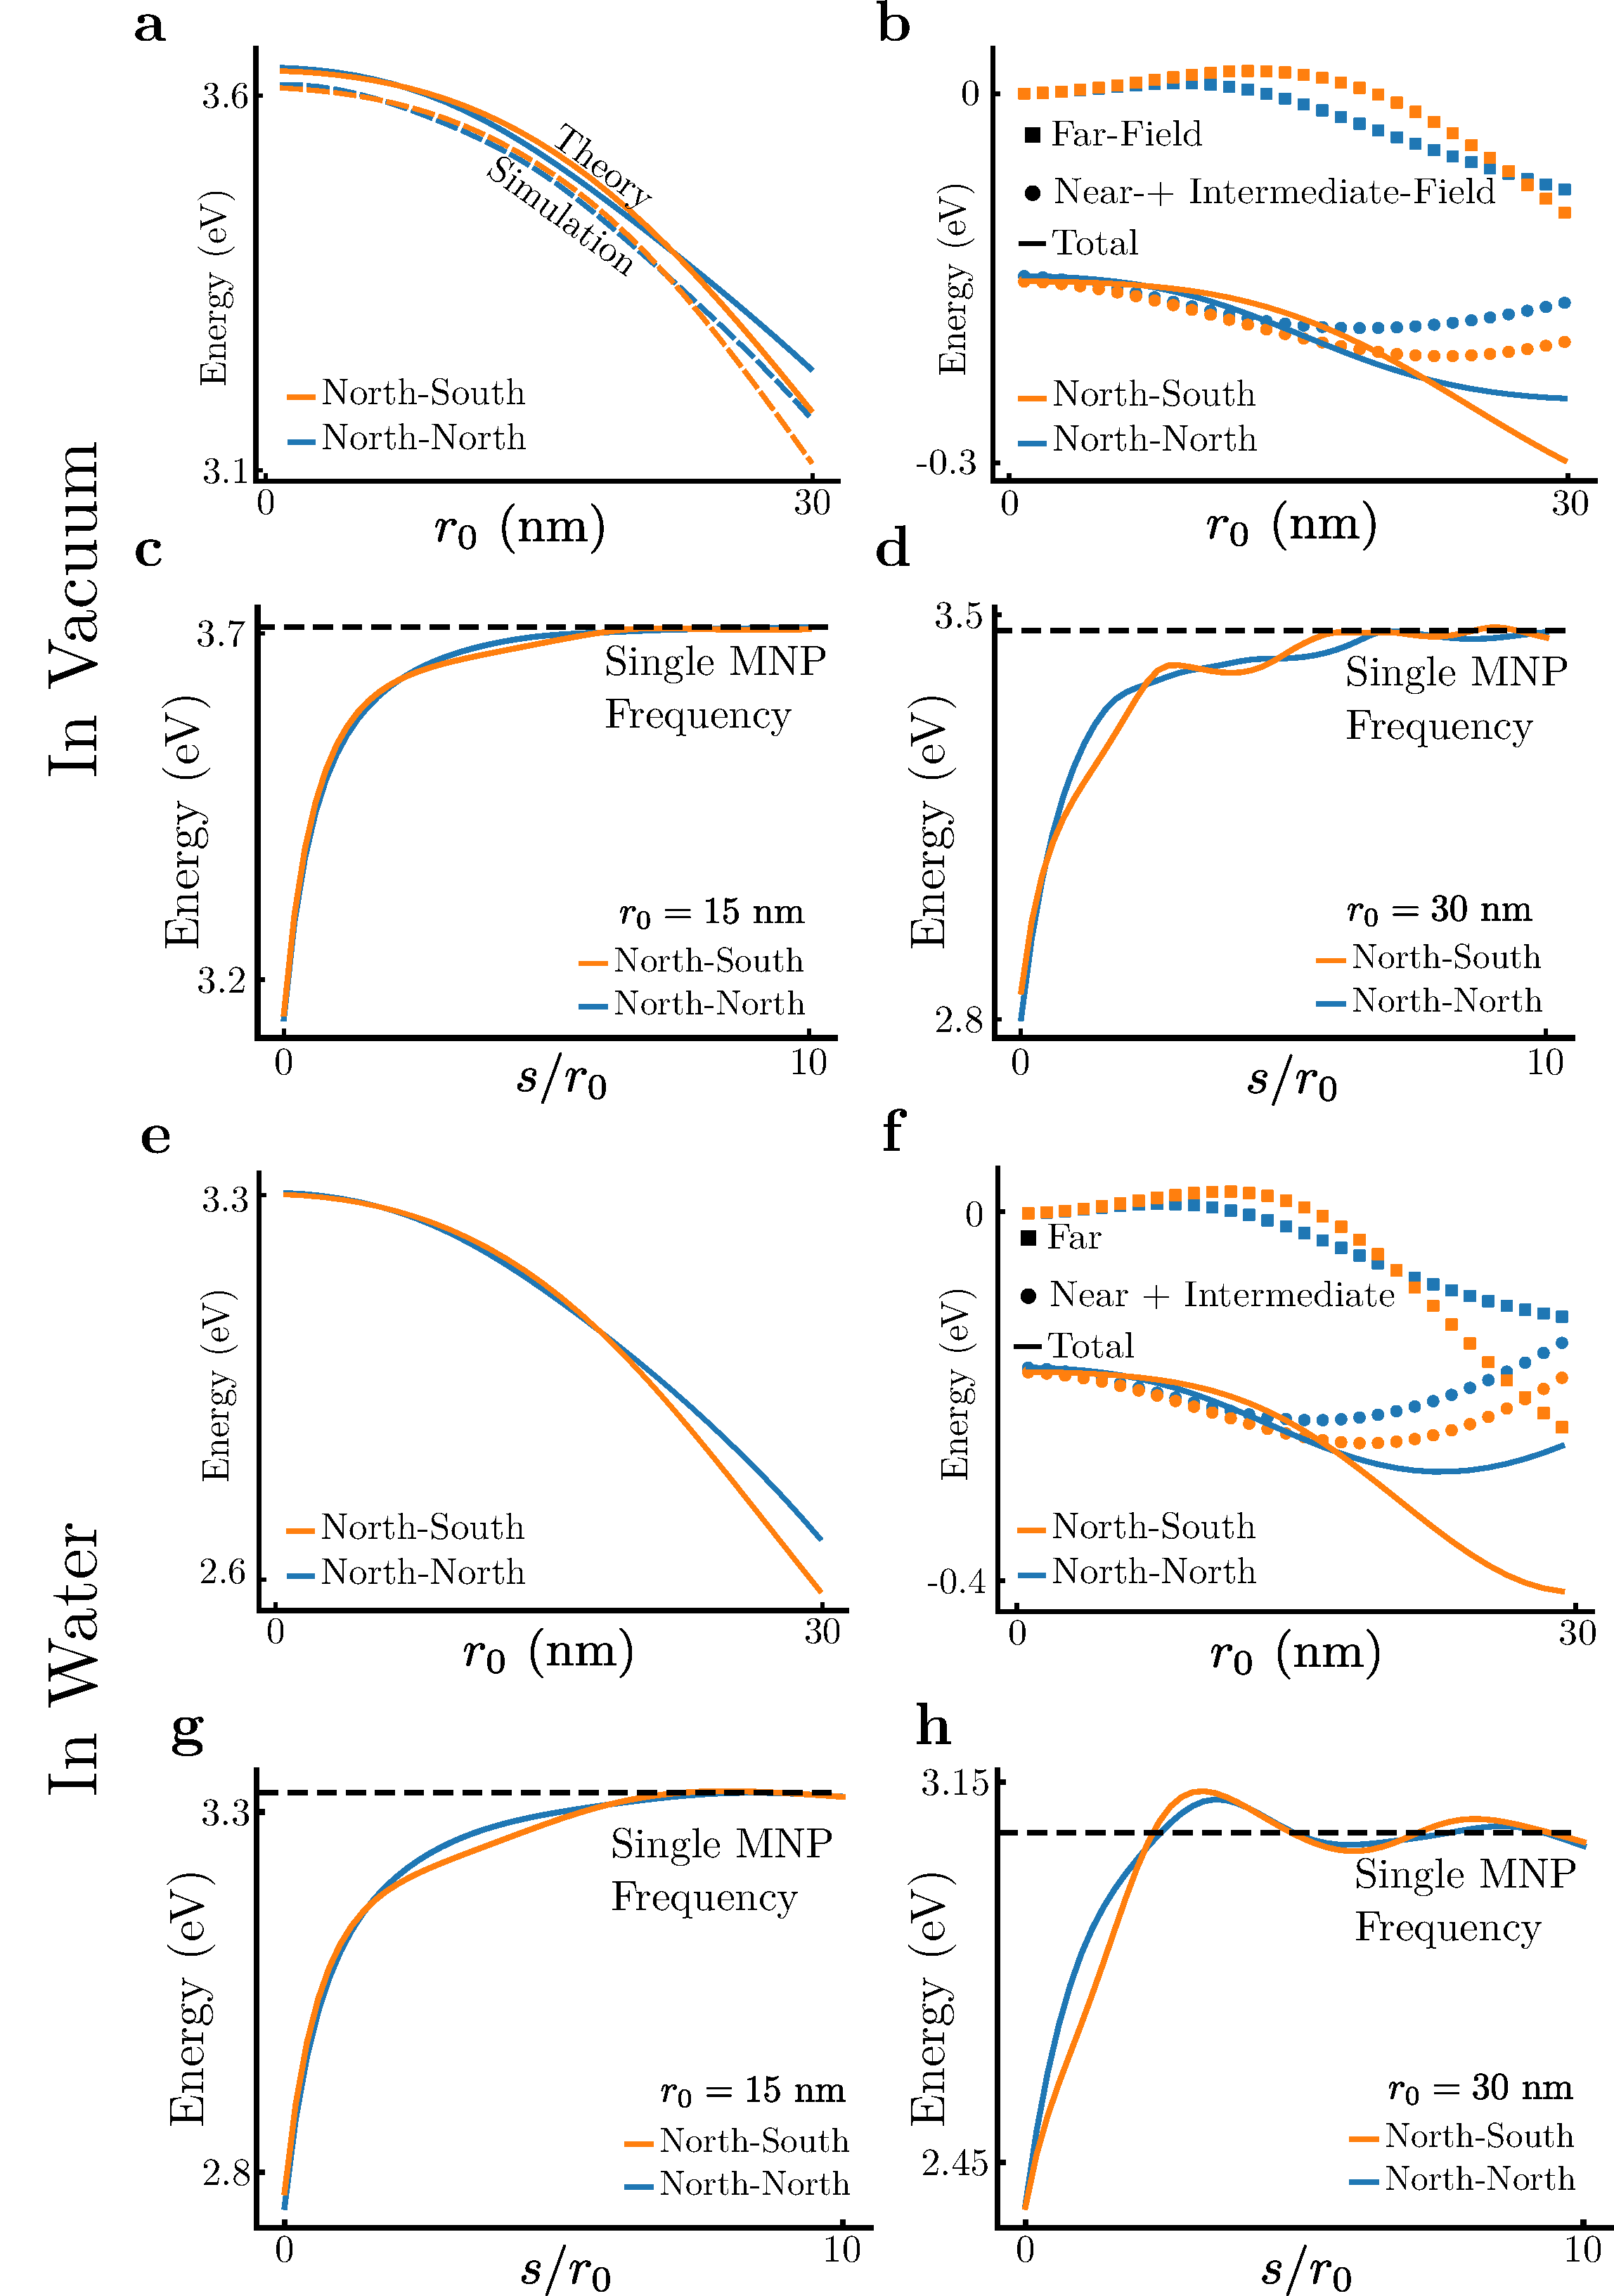
\includegraphics[width=4in]{2mer_eig_combined.pdf}
\caption{Eigenvalues and interaction energies as functions of total aggregate scale and interparticle distance for the magnetic modes of the 2mer. (a) The eigenvalues of the North-South (orange) and North-North (blue) modes for $r_0 = $ 1 to 30 nm computed using the equations of motion (solid) and compared with full-wave simulations (dashed). Note the agreement to within 0.05 eV. The modes cross twice, once at around 7 nm and a second time at around 20 nm. (b) Total (solid), near- plus intermediate-field (circles), and far-field (squares) interaction energies for each mode as a function of increasing $r_0$. The splitting between the interaction energies in the far-field has the opposite sign as in the near- and intermeidate-field, resulting in the eigenmodes crossing. (c) and (d) Magnetic mode eigenvalues as a function of increasing interparticle distance, with $r_0 =$ 15 and 30 nm, respectively. With increasing spacing, the eigenvalues tend towards the noninteracting, single-particle frequency and exhibit large oscillations and splittings. (e-h) Eigenvalues and interaction energies computed in a similar fashion to (a-d), with $\varepsilon_b = 1.77$, the dielectric constant of water.}
\label{scaling}
\end{figure}

While good for theoretical studies of system properties, scale is not tunable in real time, meaning these properties can't be easily measured. Recent research has focused heavily on finding controllable and reversible ways to manipulate the aggregation scheme of a metal nanoparticle array using tools like DNA, polymers, and stretchable embedding media\cite{Yang2016,Ginger2017,NaLiu2017,DanLuo2009}. We employ this idea by fixing the particle radii and the aggregation scheme of the structure and inflating the interparticle distances. Figure~\ref{scaling}e-h shows the results of fixing $r_0$ at 15 and 30 nm and increasing $s$. Increasing the distance between particles regardless of particle size and environment weakens the coupling as the distance approaches infinity, which can be seen in Equation~\ref{electric_field_lambda}. As a result, the collective frequencies of the magnetic modes approach the single plasmon frequency. On the way, the modes oscillate about each other, exhibiting multiple crossings. The amplitude of these crossings appears to increase with increasing particle size and with increasing background dielectric constant, which can be seen in Figure~\ref{scaling}f and h. The quasistatic approximation cannot explain this phenomenon. The fully retarded electric field contains a complex exponential term that depends on interparticle separation. It is this term that dresses all of the interaction terms in the field and changes the sign of the interaction from negative to positive at certain distances. This is clear evidence that the magnetic modes of the 2-mer are tunable in real time in a laboratory with splittings as small as 0.01 eV and as large as 0.1 eV. 

The concept of magnetic plasmons switching spectral order has not been discussed in the literature. This is likely because the splittings between the modes in the systems analyzed are smaller than the spectral resolution of most detection methods, including scattering experiments and STEM/EELS. Additionally, magnetic oligomers exhibit many other electrically bright modes that are close in energy and broad, which tends to wash out most spectra. In order to make magnetic oligomers useful, either the modes must be made fewer and more narrow, or techniques must be found that can identify and utilize the modes regardless of breadth. One such method is the measurement of directional or angle-resolved scattering.

\section{Angle-Resolved Cathodoluminescence Studies on the 2mer}
Electron beam spectroscopies, such as EELS and CL, conducted in a STEM are very useful for high spatial and spectral reoslution studies of nanomaterials. While EELS measures the probability that a passing electron loses energy to the material, CL measures the probability that the material's excited behavior results in photon emission. Recent studies have demonstrated the utility of angle-resolved CL spectroscopy to characterize a material. Using a STEM fitted with a parabolic mirror over the sample, the user can collect emitted light with angular information within $0 \leq \theta \leq \pi/2$ and $0 \leq \phi \leq \pi$. Here we show that with the selection rules imposed by the location of the electron beam and the specific directionality of the emission from each magnetic mode, the magnetic modes and their crossing can be observed in spectra.

Some figures and discussion.

\section{Angle-Resolved Cathodolumiescence Studies on the 3mer}
As we have seen in the section I haven't finished writing, the 3mer resembling a phenalene molecule supports not only an all-North magnetic plasmon, but two degenerate, orthogonal North-South magnetic plasmons as well. This is due to its threefold symmetry axis, or in the language of group theory, its D3h point group. Again, due to their different polarizations, the all-North mode can be distinguished from the North-South modes using angle-resolved CL spectroscopy.

Some figures and discussion.

\section{Now that we're done proving it to you, here are some systems that people are making right now!}
Data from Kagan paper. Emphasize where the magnetic dipole plasmon shows up. (Not always the lowest, but never as far away as the Kagan paper predicts.)

Some figures and discussion.

\section{Directional Scattering in the 2-mer}
It has been predicted and shown experimentally that single magnetic oligomers scatter light anisotropically when both their magnetic dipole and their electric dipole are excited by light.\cite{Dionne2011,Cherqui2016} This is evident from the difference between forward and backward scattering spectra, but can also be shown by computing the differential scattering pattern,\cite{jackson_classical_1999,schwinger1998classical}

\begin{equation}
\frac{dP}{d\Omega} = \frac{c}{8\pi}\left[r^2\hat{\textbf{n}}\cdot\sum_i\textbf{E}_i \times \sum_{j}\textbf{B}_{j}^*\right]
\label{dp_field_1}
\end{equation}


\begin{figure}
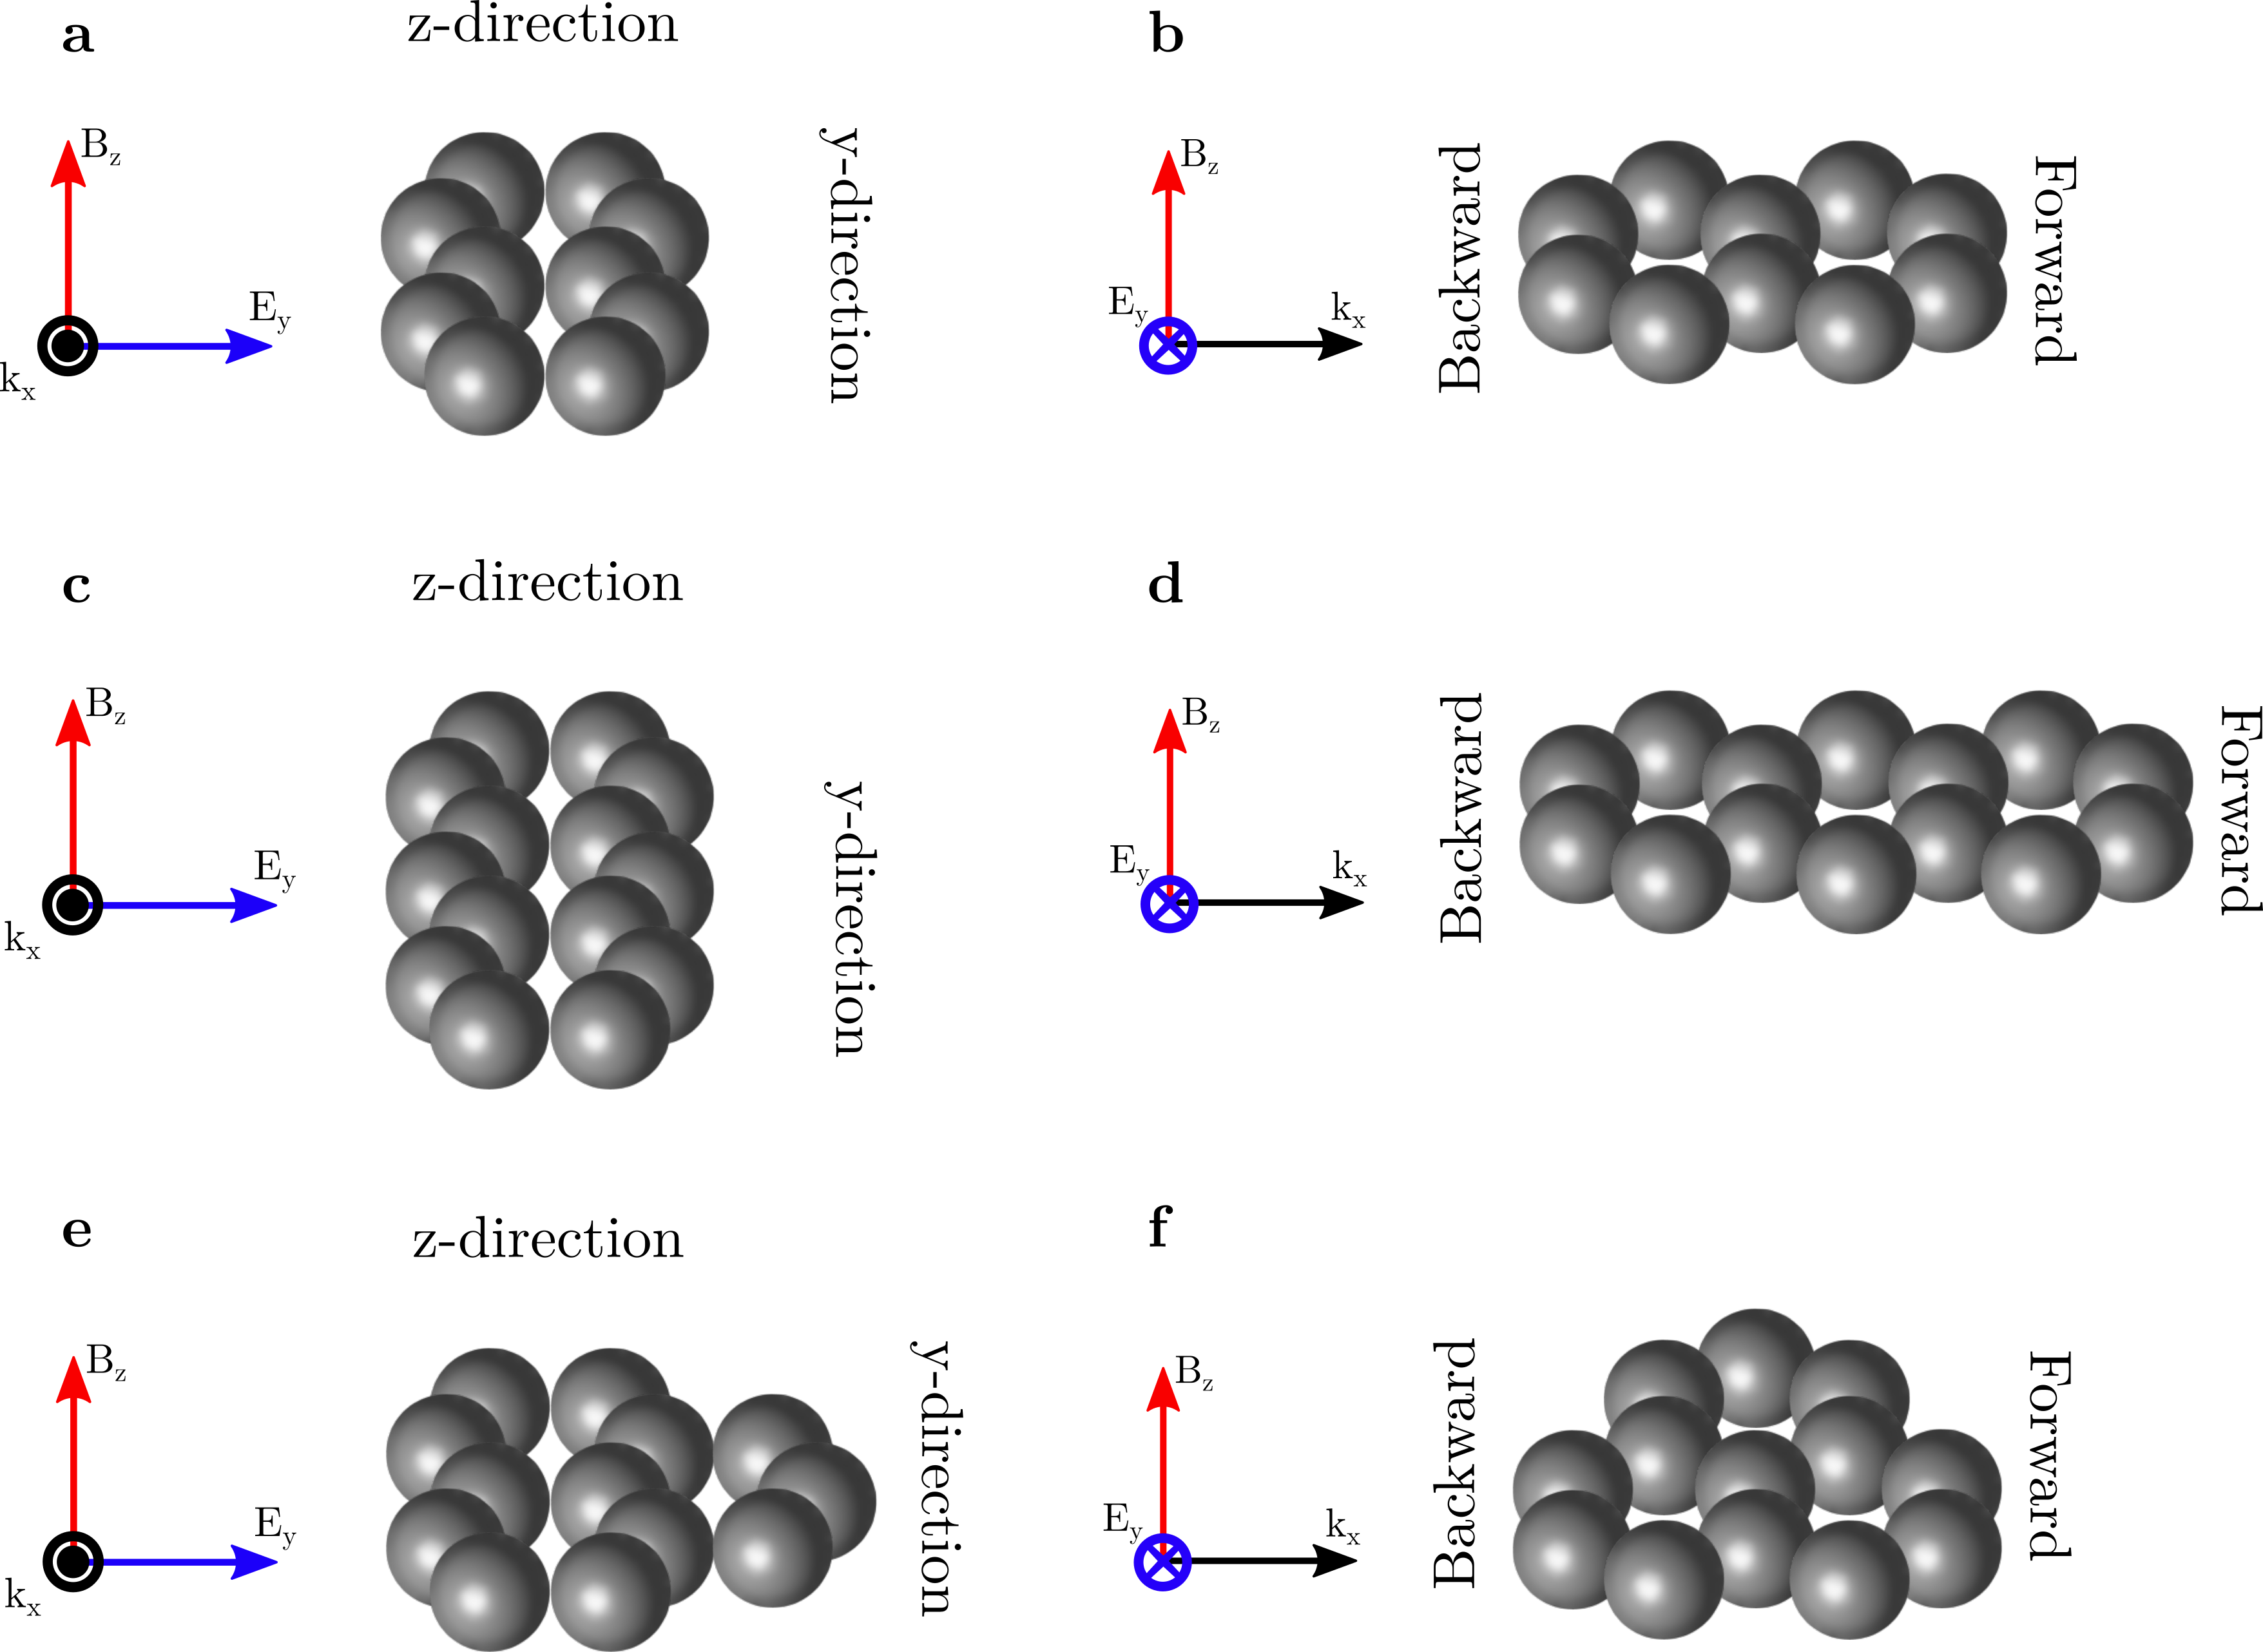
\includegraphics[width=5in]{scattering_diagrams.png}
\caption{Diagrams of the incident light and orientation of the (a and b) 2mer, (c and d) linear 3mer, and (e and f) triangular 3mer systems to be referenced with Figures~\ref{yz_scattering},~\ref{xz_scattering},~\ref{l3mer_combined}, and~\ref{t3mer_forback}.}
\label{diagrams}
\end{figure}


\noindent where $\hat{\textbf{n}}$ is the unit vector pointing to the detector a distance $r >> \lambda$ away and $\textbf{E}_i$ and $\textbf{B}_j^*$ are the electric field and conjugate magnetic inductance of the interfering collective modes of the 2mer. From here, we perform full-wave simulations to compute scattering spectra and differential scattering patterns on the 2mer and 3mers.\cite{Hohenester2012} According to the diagram in Figure~\ref{diagrams}a and b, the incident light is polarized such that the magnetic field threads the rings of the 2mer, while the electric fieldpoints along its short axis. Using the far-fields scattered by these collective dipole moments, and subsittuting them into Equation~\ref{dp_field_1}, the differential scattering becomes\cite{Engheta2006}

\begin{equation}
\frac{dP}{d\Omega} = \frac{ck^4N^2}{4\pi}\left[|\textbf{d}_{e}|^2(1-(\hat{\textbf{n}}\cdot\hat{\textbf{y}})^2) + k^2R^2|\textbf{d}_{m}|^2(1-(\hat{\textbf{n}}\cdot\hat{\textbf{z}})^2) + kR(\textbf{d}_{e}\cdot\textbf{d}_{m}^* +\textbf{d}_{e}^*\cdot\textbf{d}_{m})(\hat{\textbf{n}}\cdot\hat{\textbf{x}})\right].
\label{dp_dipoles_1}
\end{equation}

\noindent Here, $N$ is the number of particles in an aggregate, $\textbf{d}_e$ is the electric dipole moment of a single particle in the collective electric mode, $\textbf{d}_m$ is the electric dipole moment of a single particle in the collective magnetic mode, and $R$ is the radius of a cluster. In the case that $d_m = 0$, the second and third terms vanish, resulting in a scattering pattern traditionally associated with a dipole oriented in the y-direction. When $d_e = 0$, the first and third terms vanish, and the same pattern is recovered but in the z-direction. Finally, when both sets of dipole moments are non-zero, the third term contributes an overall asymmetry in the x-direction, which here is the light propagation direction. This means that when the collective electric and the collective magentic mode interfere when both are excited simultaneously. We use this model to gain intuition about and explain the results of the simulated differential scattering patterns.

\begin{figure}
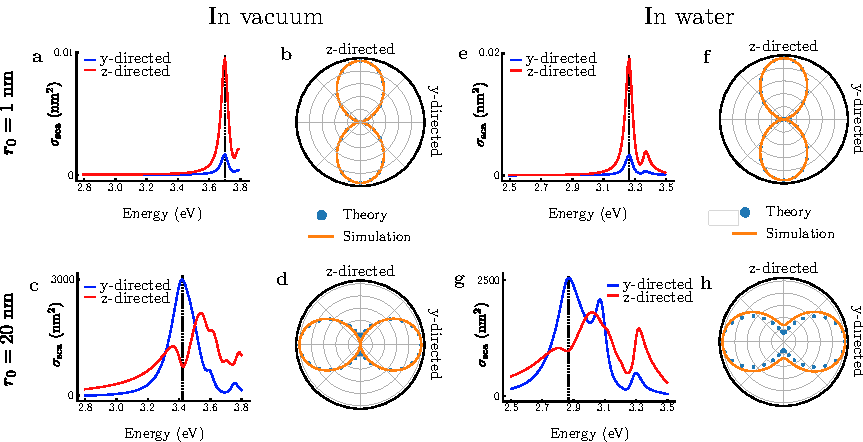
\includegraphics[width=5.5in]{yz_scat.pdf}
\caption{Scattering spectra and differential scattering patterns for the 2mer in vacuum and in water. (a) Scattering spectrum for the 2mer with $r_0 =$ 1 nm and $s = 1$ displaying z-directed (red) and y-directed (blue) scattering. (b) Differential scattering pattern verifying that the z-directed scattering is much larger than the y-directed scattering. (c) Scattering spectrum for the 2mer with $r_0 =$ 20 nm and $s=1$, again with z-directed (red) and y-directed (blue) light. (d) Differential scattering pattern veryifying that at the chosen frequency, the y-directed scattering is greater than the z-directed scattering. (e-h) Scattering calculations in the same fashion as (a-d), with $\varepsilon_b = 1.77$, the dielectric constant of water.}
\label{yz_scattering}
\end{figure}

Analyzing first the y- and z-oriented scattering gives a measure of the relative strength of the electric and magnetic modes. When $d_e >> d_m$ the y-directed scattering should approach zero while the z-oriented scattering will be maximized. This can be seen quite clearly in Figure~\ref{yz_scattering}a and b, where the electric dipole mode's dominance is evident through the primarily z-oriented scattering, especially at the peak frequency (dashed black line). As discussed previously, when the oligomers are small they behave quasistatically with almost no magnetic effects, so it is expected that the purely electric physics should dominate. Figure~\ref{yz_scattering}c and d shows that at larger sizes the dominance of either y- or z-directed scattering is frequency dependent, signifying that the magnetic dipole moment can dominate the scattered light at certain frequencies. The scattering pattern in (d) corresponds to the black dashed line in (c), emphasizing the frequency at which the magnetic dipole is strongest compared to the electric dipoles. This shows that magnetic oligomers scatter light of certain colors in different directions. While Equation~\ref{dp_dipoles_1} suggests through its $R$-dependence that at large sizes the magnetic dipole moment should dominate the scattering, the presence of the individual dipole moments suggests a dependence on the oscillator strength of the collective modes. At the resonant frequency of the magnetic mode, it dominates the scattering pattern, but at other frequencies the electric dipole modes dominate. This suggests that the magnetic mode is much narrower and harder to force than the electric modes. This is interesting because this implies a method of detecting the frequency at which the all-North magnetic mode significantly impacts the optical properties of a given magnetic oligomer. Further emphasizing this is the fact that increasing the spacing between the particles shifts the resonances to higher energy, so probing at the same frequency results in a different scattering pattern, as depicted in [\textbf{Figure not done yet!}]. This offers a way to controllably choose the directionality of specific colors of light by manipulating the aggregation scheme of magnetic oligomers. These results are consistent in water as well, as shown in Figure~\ref{yz_scattering}e-h.

Using the y- and z-directed scattering to understand the relative strength of the magnetic and electric dipole moments is only one side of the story. Looking instead at the x- and z-directed scattering opens up a tool to quantify the extent to which electric and magnetic plasmons interfere with one another. As suggested by the third term of Equation~\ref{dp_dipoles_1}, in the direction of propagation we should expect to see asymmetry when both the electric dipole moment and magnetic dipole moment are of appreciable magnitude. Figure~\ref{xz_scattering} shows spectra computed in the forward and backward direction for particles of $r_0 = $ 1 nm and 20 nm (a and c) as well as differential scattering patterns in the xz-plane (b and d) in vacuum, and similarly in water (e-h). The differential scattering patterns have been computed at the frequencies that maximize the forward-to-backward ratio. As suggested by the $R$-dependence and the dependence on dipole strength in Equation~\ref{dp_dipoles_1}, at small sizes the radiation is isotropic in the forward (red) and backward (blue) direction. This again makes sense, as small oligomers are dominated by electric near-field effects. However, with increasing size, the interference term in Equation~\ref{dp_dipoles_1} begins to influence the spectrum and the scattering, leading to a large amount of directional radiation. Like before, this is dependent upon not only the size of the system but upon the oscillator strength of each mode, and so probing off resonance of the magnetic mode diminshes its influence and leads to more significant backward-directed radiation. However, at all frequencies the forward scattering is larger than the backward scattering, and even upon changing the interparticle distance this remains true. This suggests that once the magnetic mode is strong and broad enough to interfere with the electric modes, the directional radiation can not be completely turned off except by moving the particles infinitely far away from each other. Furthermore, this must be a collective effect as the constituent particles here are too small to exhibit appreciable magnetic moments and radiate unidirectionally by themselves. Magnetic dipole-electric dipole scattering interference has been predicted and observed in metal-dielectric core-shell systems and single magnetic oligomer systems, and directional or angle-resolved scattering experiments are common practice on metal nanoparticle aggregates.\cite{Dionne2011,Kivshar2012,Polman2014,Smith2014,Tsutomu2017}

\begin{figure}
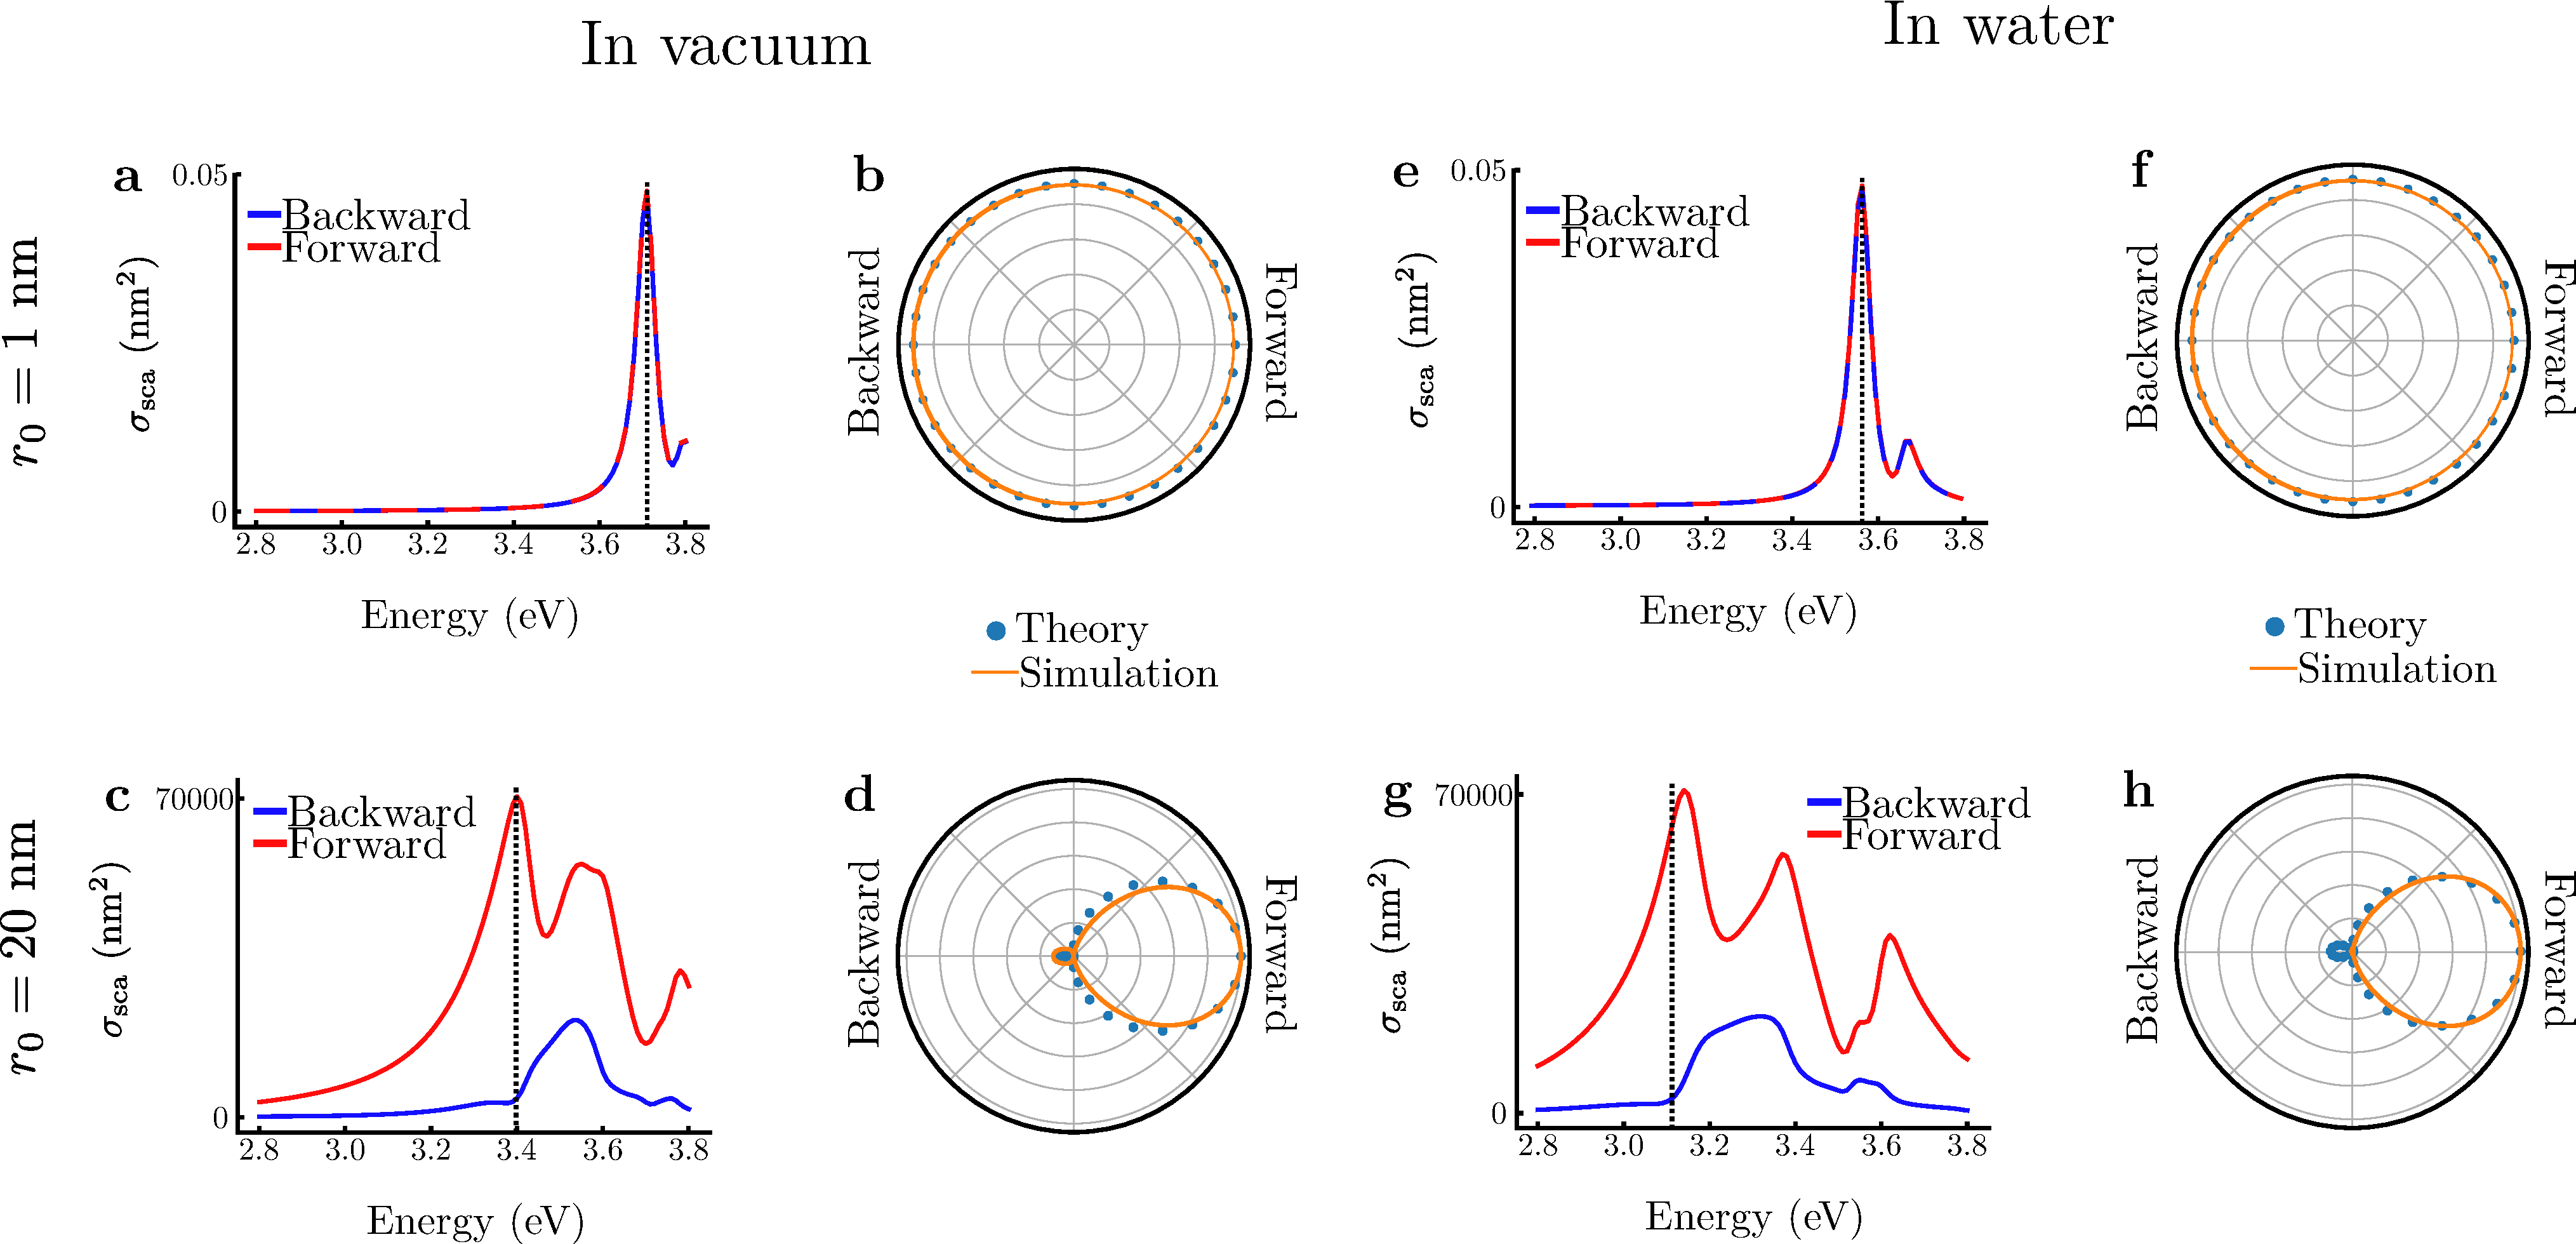
\includegraphics[width=5.5in]{for_back_spectra.pdf}
\caption{Forward and backward scattering spectra and differential scattering patterns for the 2mer. (a) Forward (red) and backward (blue) scattering spectra for the 2mer with $r_0 =$ 1 nm and $s=1$ nearly overlap. (b) The isotropic radiation pattern in the forward and backward direction computed using the model in Equation~\ref{dp_dipoles_1} (blue dots) and full-wave simulations (orange line). (c) Forward (red) and backward (blue) scattering spectra for the 2mer with $r_0 =$ 20 nm and $s=1$ are vastly different, showing that the forward scattering is almost always greater than the backward scattering. (d) The differential scattering pattern at the frequency marked by the dashed line in (c) shows that the scattering is nearly unidirectional both using the model (blue dots) and simulations (orange). (e-h) Scattering spectra and patterns computed in the same way as (a-d), except with $\varepsilon = 1.77$.}
\label{xz_scattering}
\end{figure}

\section{Methods}
Here we show how to derive the equations of motion, and solve an example system of two coupled oscillators. The Hamiltonian for a system of $N$ coupled oscillators

\begin{equation}
H = \sum_{i}\frac{\textbf{p}_i^2}{2m_{\textrm{sp}}}+\frac{1}{2}m_{\textrm{sp}}\omega_{\textrm{sp}}^2\textbf{q}_i^2 - \frac{e}{2}\sum_{j\neq i}\textbf{q}_i\cdot\textbf{E}_j(\textbf{r}_i),
\label{hammy}
\end{equation}

\noindent where $\textbf{p}_i$ are the momenta of the plasmon oscillators with coordinates $\textbf{q}_i$, $m_{\textrm{sp}}$ is the plasmon mass, $\omega_{\textrm{sp}}$ is the plasmon frequency, and $\textbf{E}_j(\textbf{r}_i)$ is defined in Equation~\ref{electric_field_lambda}. The next step is to write Hamilton's equations of motion,

\begin{equation}
\dot{\textbf{p}}_i = -\frac{\partial H}{\partial\textbf{q}_i} = -m_{\textrm{sp}}\omega_{\textrm{sp}}^2\textbf{q}_i + e\sum_{j\neq i}\textbf{E}_j(\textbf{r}_i)
\label{p_dot}
\end{equation}

\noindent and

\begin{equation}
\dot{\textbf{q}}_i = \frac{\partial H}{\partial\textbf{p}_i} = \frac{\textbf{p}_i}{m_{\textrm{sp}}}.
\label{q_dot}
\end{equation}

Finally, taking another time derivative of Equation~\ref{q_dot} and plugging in Equation~\ref{p_dot}, we obtain the equation of motion

\begin{equation}
\ddot{\textbf{q}}_i = -\omega_{\textrm{sp}}^2\textbf{q}_i + \frac{e}{m_{\textrm{sp}}}\sum_{j\neq i}\textbf{E}_j(\text\
bf{r}_i)
\label{equation_of_motion_again}
\end{equation}

\noindent which is exactly Equation~\ref{equation_of_motion}. From here, introducing time-dependence as a complex exponential, rewriting the electric field in terms of the plasmon coordinate, and performing a Fourier transform results in equations of motion in the frequency domain

\begin{equation}
(\omega_{\textrm{sp}}^2-\omega^2)\textbf{q}_i -\frac{e^2}{m_\textrm{sp}}\sum_{j\neq i}\boldsymbol{\Lambda}_{ij}\cdot\textbf{q}_j = 0.
\label{fourier_eom}
\end{equation}

It is this system of equations for the plasmon oscillator coordinates that we solve for the normal modes. As an example, we demonstrate this calculation for two coupled oscillators displaced and oriented along the x-axis. Knowing the dipole orientation allows us to project out the vector components and reduce the coupling term to a constant, resulting in

\begin{equation}
(\omega_{\textrm{sp}}^2-\omega^2)q_1 -g_{1,2}q_2 = 0
\label{fourier_eom_1}
\end{equation}

and

\begin{equation}
(\omega_{\textrm{sp}}^2-\omega^2)q_2 -g_{1,2}q_1 = 0.
\label{fourier_eom_2}
\end{equation}

Putting these equations of motion in matrix form allows us to solve for the eigenvalues and eigenvectors as follows.

\begin{equation}
\begin{bmatrix}
(\omega_{\textrm{sp}}^2-\omega^2) & -g_{1,2}\\
-g_{1,2} & (\omega_{\textrm{sp}}^2-\omega^2)
\end{bmatrix}
\begin{bmatrix}
q_1\\
q_2
\end{bmatrix}
=
\begin{bmatrix}
0\\
0
\end{bmatrix}
\label{eom_matrix}
\end{equation}

Finding the determinant of this matrix yields the eigenvalues of the collective modes,

\begin{equation}
\omega_{\pm} = \sqrt{\omega_{sp}^2 \pm g_{1,2}}.
\label{eigenvalues}
\end{equation}

\noindent Of course, the coupling terms $g_{1,2}$ in fact depend on the frequency of the collective mode, which is demonstrated in Equation~\ref{electric_field_lambda}. Because of this, the eigenvalue problem must be solved iteratively until the eigenvalues converge. This example can be extended to systems of an arbitrary number of dipoles, and this exact method is used to solve for the eigenvalues of the magnetic plasmon modes.

\section{Eigenvalue Calculations on the 3mers}
\begin{figure}
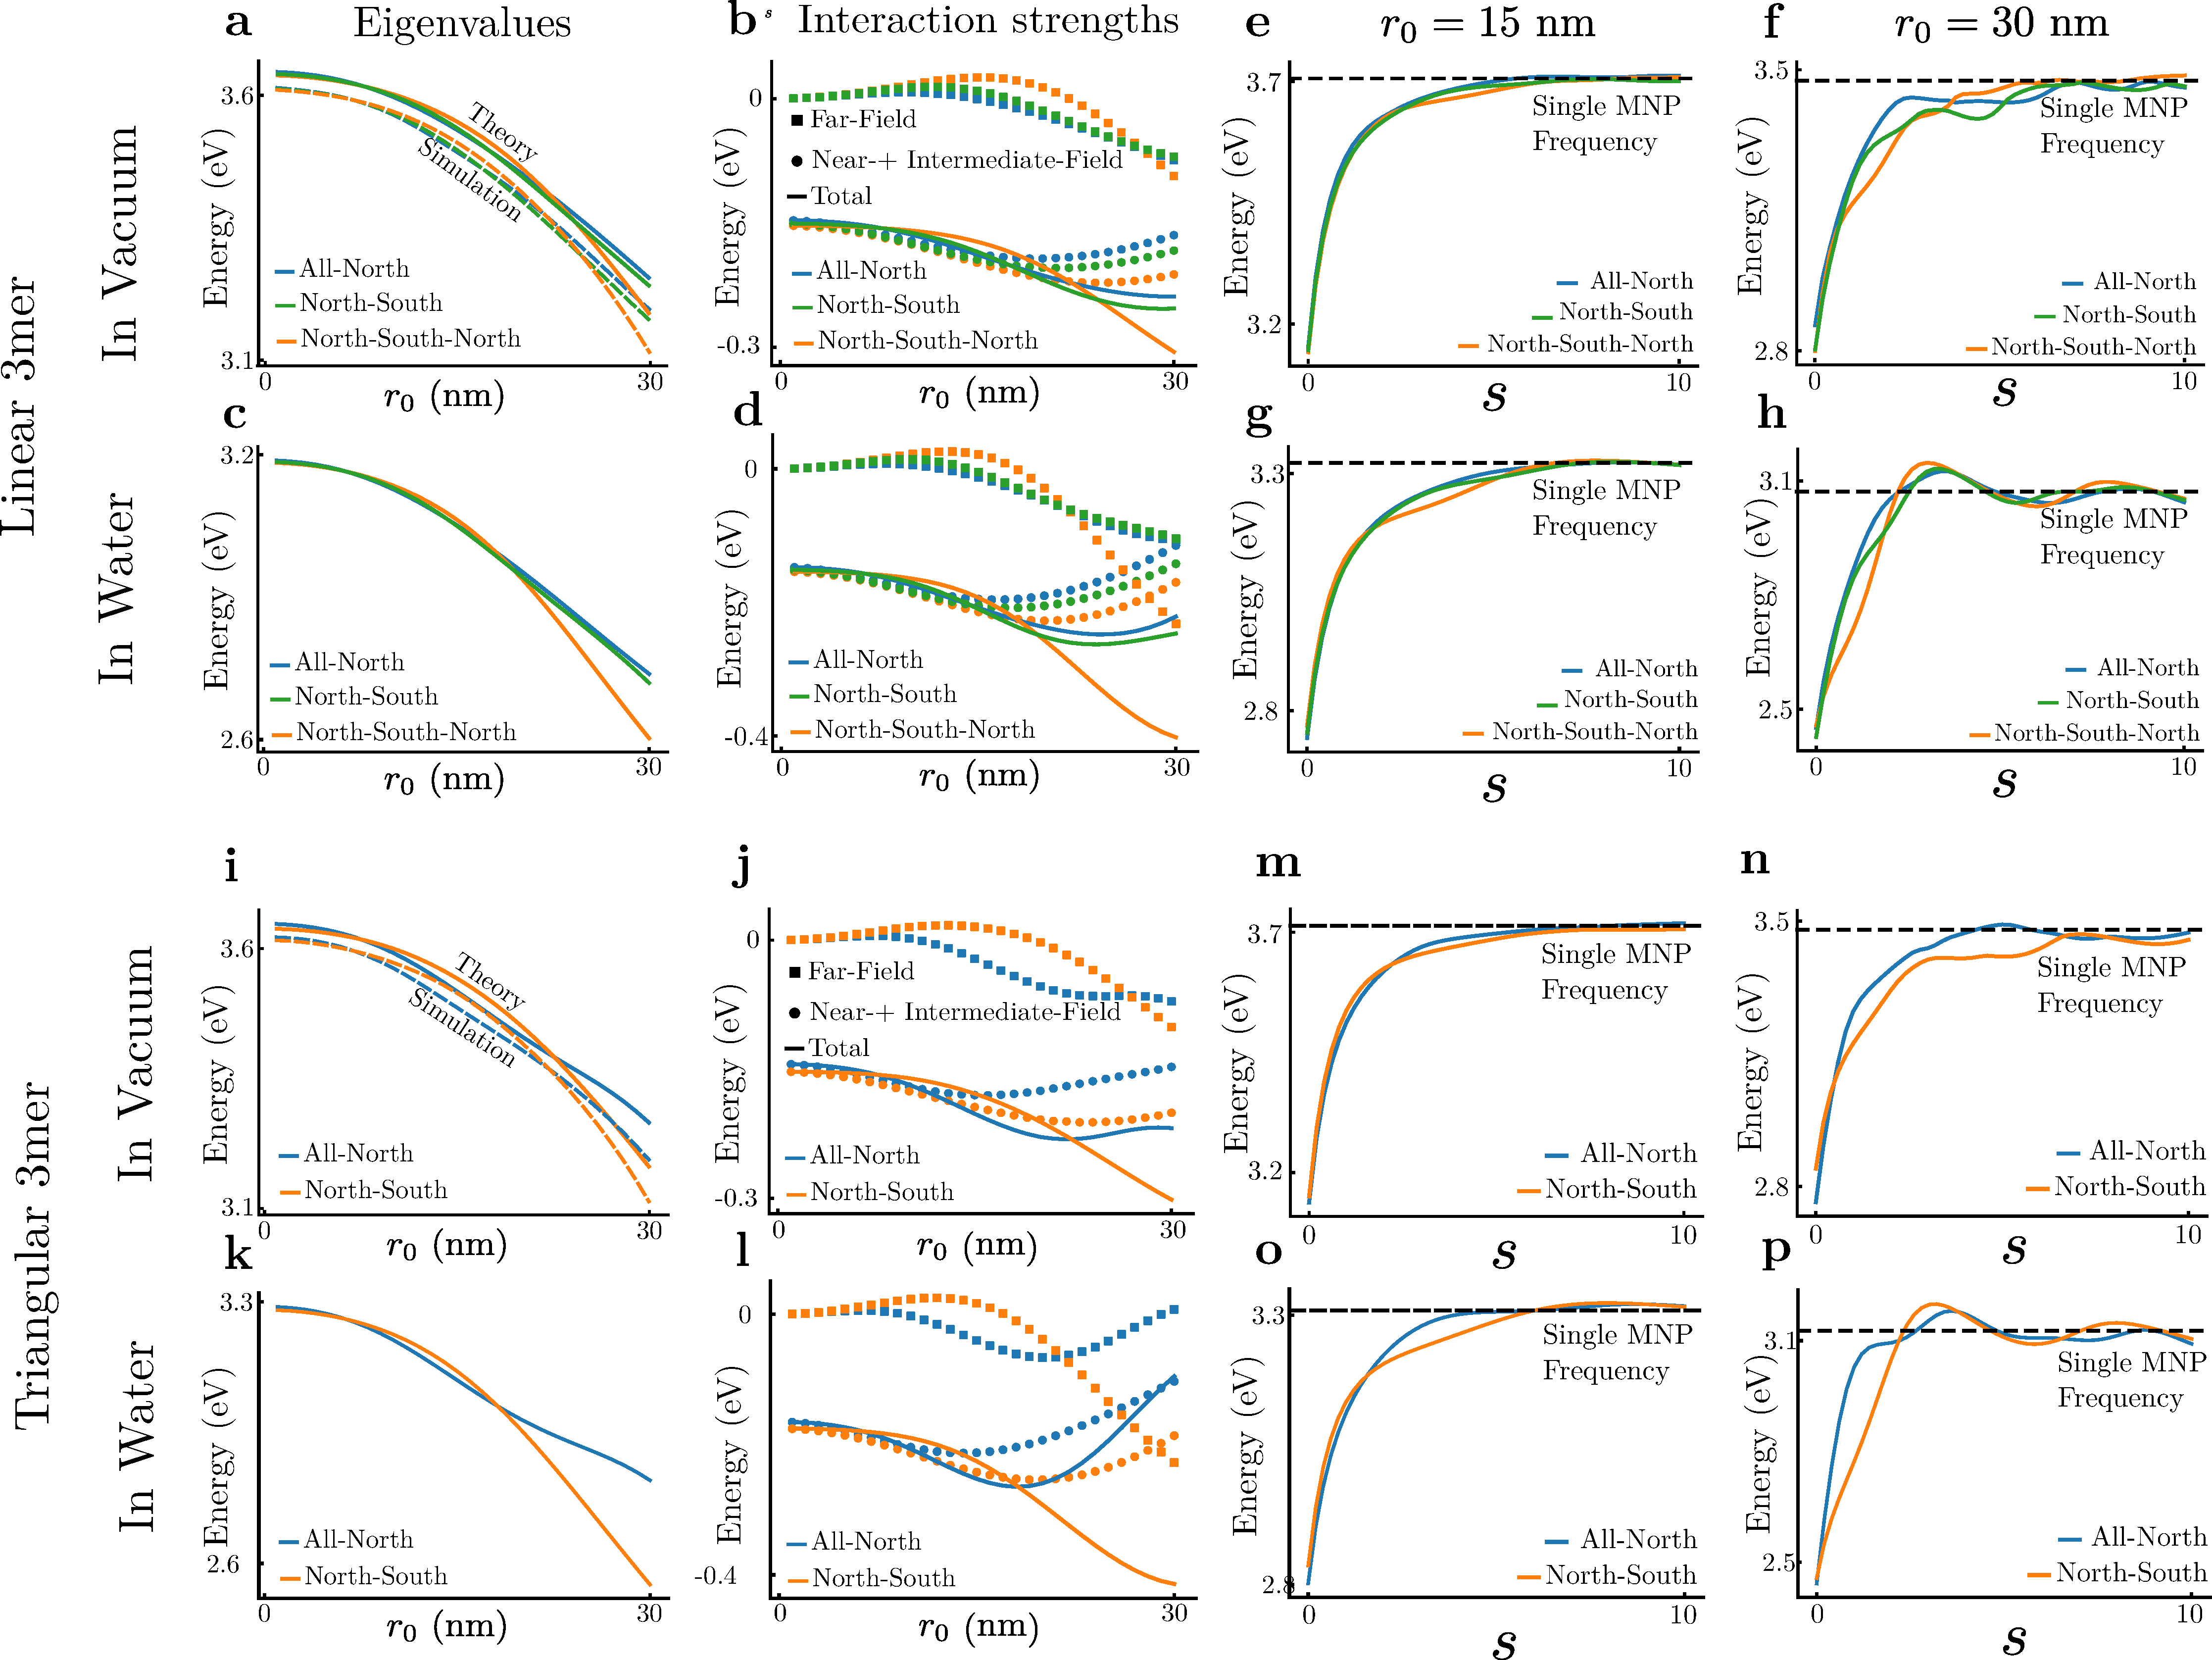
\includegraphics[width=5in]{3mer_eig_combined.pdf}
\caption{Eigenvalues and interaction energies of the magnetic modes of both the linear and triangular 3mers in vacuum and water. (a) The eigenvalues computed from the model on the three modes of the linear 3mer, showing crossing points at around 7.5 nm and 21 nm and compared with simulation results (dashed lines). (b) Interaction energies computed from Equation~\ref{interactionenergy}, with the far-field (squares) being entirely responsible for the crossing points in (a) while the near- and intermediate-field terms (circles) contribute only a net shift to the total (solid) interaction. (c and d) Similar plots to (a and b) with a background of water, which moves both crossing points to smaller size. (e) Eigenvalues as a function of interparticle spacing for particles of radius 15 nm, exhibit multiple crossings and low-amplitude oscillations when compared to larger (f) particles. (g and h) Similar results to (a and b), with a background of water, causing a net shift to lower energy of all eigenvalues and larger oscillations, but no drastic qualitative change. (i-p) Display similar results to (a-h) for the triangular 3mer. The analysis is very similar, as the eigenmodes have crossing points in similar locations and the eigenvalues and interaction energies are similarly impacted by the background of water.}
\label{3mer_eig}
\end{figure}

The model presented earlier in this paper can also be applied to the 3mer systems. Looking first at Figure~\ref{field_plots}, each 3mer supports three magnetic modes, rather than two. However, the triangular 3mer's two electric dipole modes (f and g) are degenerate. This is represented in Figure~\ref{3mer_eig}, where the plots concerning the linear 3mer have 3 traces and the plots concerning the triangular 3mer have two traces. What is interesting about this analysis is that the 3mers do not differ greatly in spectral ordering from the 2mer. The eigenvalue plots and the interaction energy plots have similar qualitative features amongst all three systems. This may be evident of a kind of saturation length to individual electric plasmon interaction, predicted in previous work.\cite{Pinchuk2016} However, for the purposes of this paper, this simply shows that the model can be extended to larger systems without loss of accuracy or efficiency. More importantly, these magnetic modes can influence the directionality of scattered light, much like those of the 2mer.

\section{Scattering Results from the 3mers}
Now that we have thoroughly analyzed the properties of the 2mer, we next present results on the two 3mers mentioned previously, whose modes and aggregation schemes were displayed in Figure~\ref{field_plots}. Calculations similar to those presented in Figure~\ref{scaling} for the linear and triangular 3mers are shown in the Supporting Information. These results show no new trends, but verify that the theoretical method works for larger aggreagtes with more complicated aggregation schemes. From here, we present scattering spectra and differential scattering patterns for both 3mers.

\begin{figure}
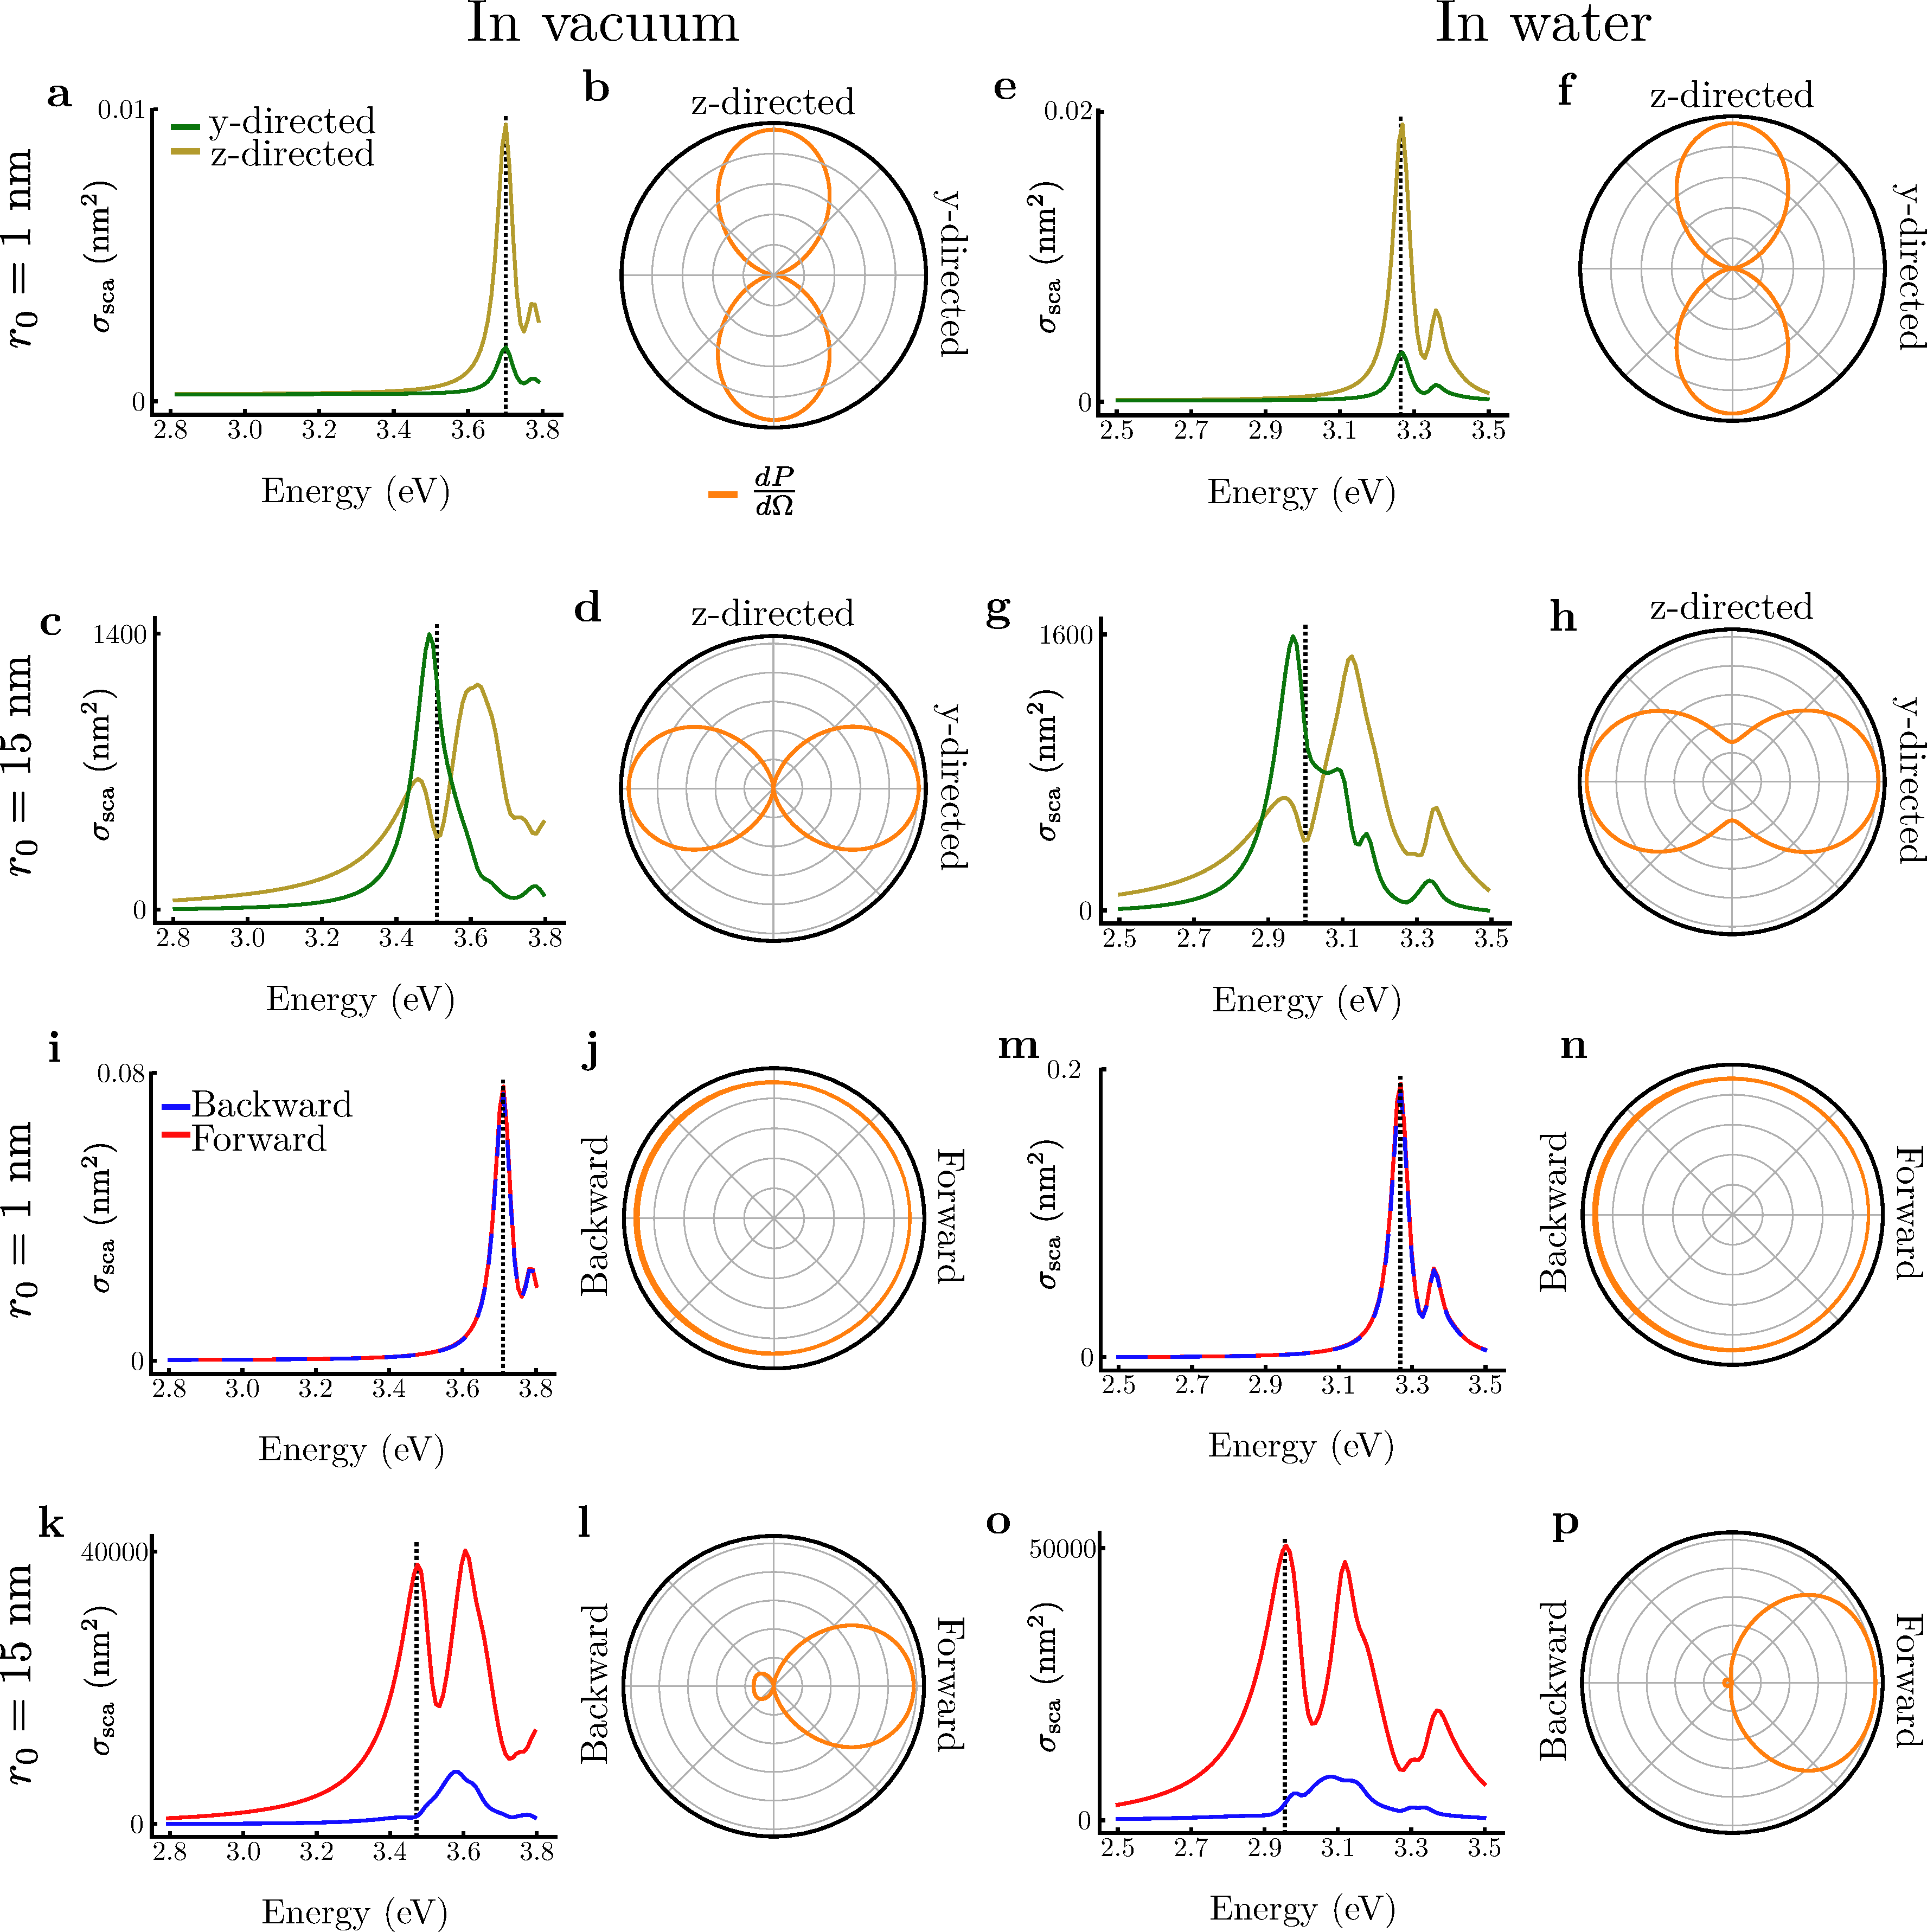
\includegraphics[width=5.5in]{l3mer_scattering_combined.pdf}
\caption{(a-h) Scattering spectra and differential scattering patterns comapring the y- (blue) and z-directed (red) scattering of the linear 3mer. (i-p) Forward (red) and backward (blue) scattering spectra and scattering patterns for the linear 3mer. (a) The y-directed scattering is much larger than the z-directed scattering for a linear 3mer with $r_0 =$ 1 nm and $s=1$, confirmed by (b) the simulated differential scattering in that plane. For a linear 3mer with $r_0 =$ 15 nm (c), the difference between the two directions depends on frequency. At the frequency marked by the dotted line, the differential scattering pattern in (d) shows that the y-directed scattering is much higher than z-directed. (e-h) Similar computations as in (a-d), except performed with a background of water. (i) The forward and backward scattering for a linear 3mer with $r_0 = $ 1 nm and $s=1$ are nearly identical, as confirmed by (j) the isotropic scattering pattern. (k) For a 3mer of larger particles, the forward scattering is greater than the backward scattering at all computed frequencies. At the frequency marked by the dotted line, (l) the diffraction pattern shows a large degree of directionality. (m-p) Similar calculations as (i-l), computed in water. }
\label{l3mer_combined}
\end{figure}

Much like the 2mer, The directionality of scattered light is a measure of how much the magnetic dipoles of the 3mers contribute to their overall optical properties. Introducing a third ring at the end of the 2mer to produce the linear 3mer does not starkly change the optical properties, except that the dominance of the magnetic mode occurs at even smaller sizes, with $r_0=$ 15 nm, as opposed to 20 nm in the 2mer. The spectra and differential scattering patterns in Figure~\ref{l3mer_combined} share a strong resemblance to those of the 2mer, showing that at small sizes, the z-directed scattering dominates and the forward and backward scattering are isotropic. This is evidence that only a net electric diple moment is exciteable on small systems. At large size, the magnetic and electric dipole moments fight for dominance at different frequencies, but at all frequencies the forward scattering is much larger than the backward scattering.

\begin{figure}
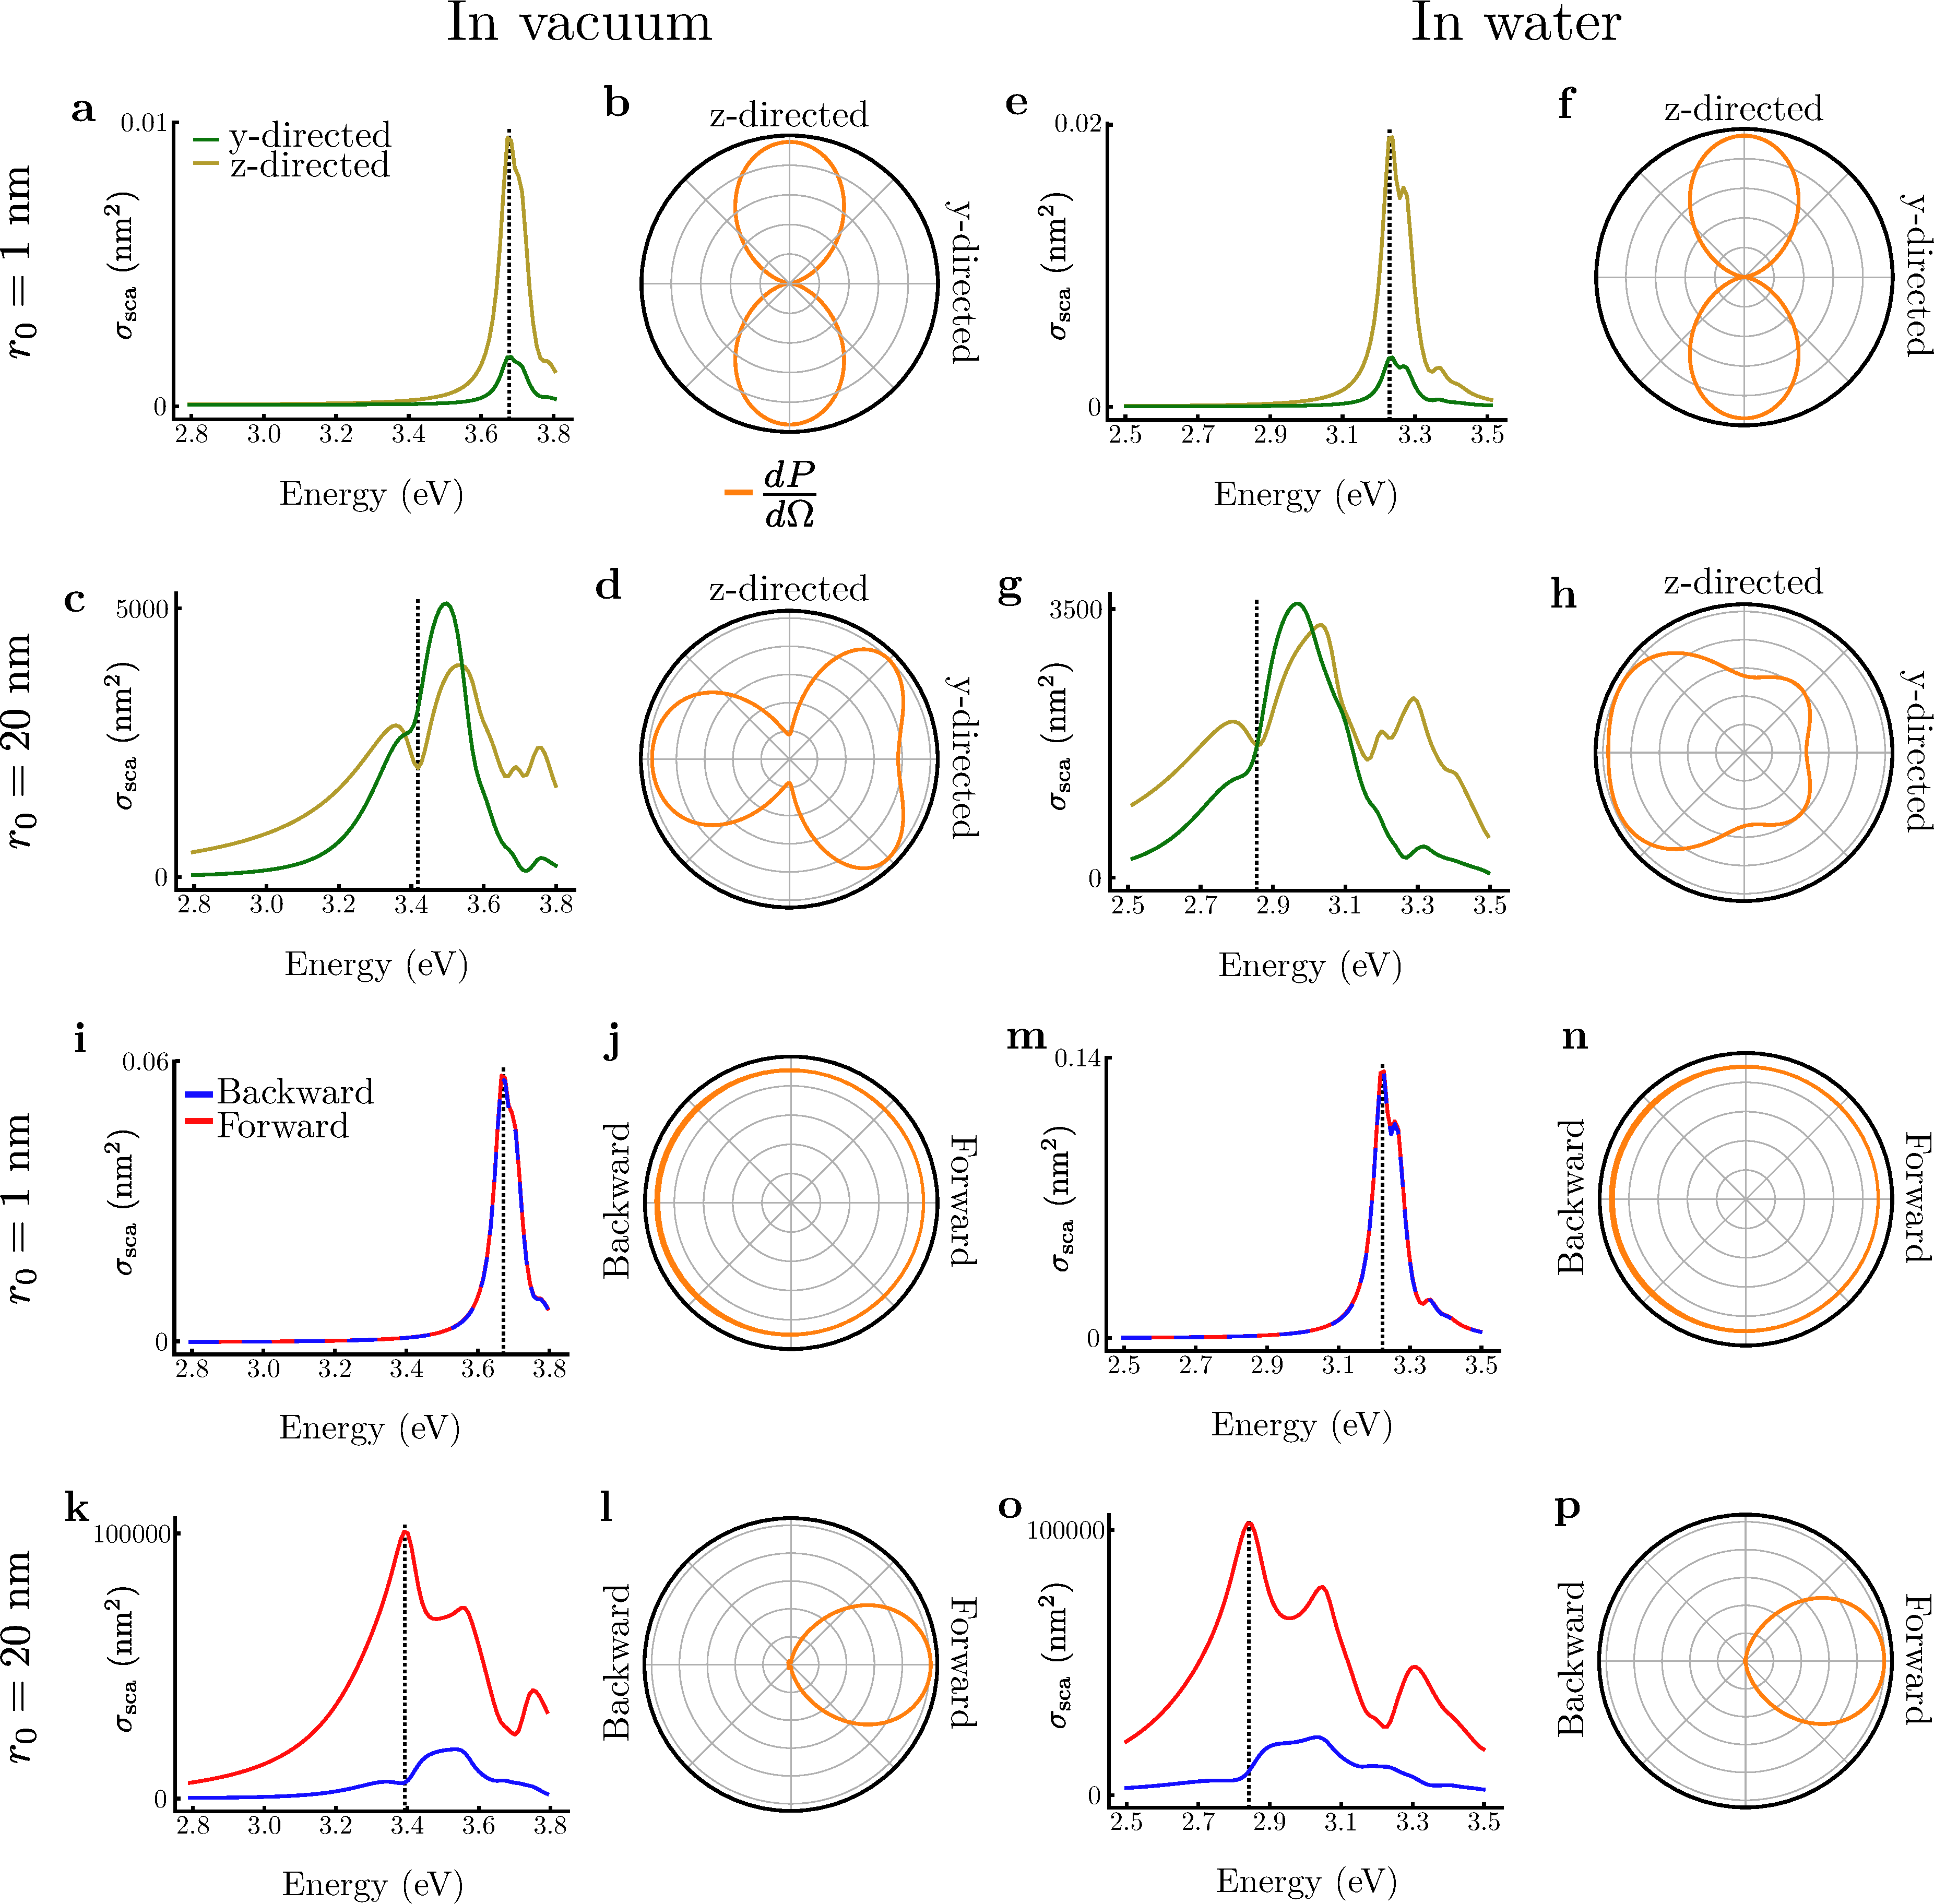
\includegraphics[width=5.5in]{t3mer_all_scattering.pdf}
\caption{Scattering spectra and differential scattering patterns computed in the y- and z-directions (a-h) and in the forward and backward directions (i-p). (a) The z-directed scattering is far greater than the y-directed scattering for the triangular 3mer with $r_0 = 1$ nm and $s=1$, owing to the excitation of only a net electric dipole moment in this size regime. This is confirmed by (b) the differential scattering pattern. (c) When the 3mer is composed of particles with $r_0 = 20$ nm, the directionality of light is frequency-dependent. Contrary to previous results, the peaks and dips in each scattering direction are uncorrelated, which is confirmed by (d) the differential scattering pattern collected at the frequency marked by the dashed line. This shows that some other collective mode of the system is weakly interfering and radiating, disrupting the symmetry expected from linear magnetic oligomers. These results are reproduced in water in (e-h). Similarly to the 2mer and the linear 3mer, (i) the forward (red) and backward (blue) scattering at small sizes are nearly equal, which is confirmed by (j) the differential scattering pattern. At larger sizes, (k and l) the triangular 3mer scatters light nearly completely unidirectionally at the chosen frequency, evidence of almost perfect interference between the magetic and electric dipole moments in the system. The results in water are qualitatively similar (m-p), showing that these properties do not drastically change in medium.}
\label{t3mer_forback}
\end{figure}

The triangular 3mers exhibit new effects that can't be explained using either the 2mer or linear 3mer for comparison. Figure~\ref{t3mer_forback} shows that at small sizes, the triangular 3mer behaves much like the 2mer and the linear 3mer, likely because it fits entirely into a wavelength of light and is too small for magentic effects to matter. However, at large sizes, the spectra and scattering patterns of the triangular 3mer do not exhibit nicely correlated peaks and dips the way that the 2mer and linear 3mer do. This is likely because of the threefold symmetry of the triangular 3mer. Previous work has shown that systems with threefold symmetry exhibit unexpected directionality in their scattered radiation.\cite{Tsutomu2017} This is likely due to the degeneracy of the dipole moments on the this 3mer and the ability to weakly excite electric dipole moments with different orientations using only one polarization of light (imagine rotating Figure~\ref{field_plots}f about a threefold axis).

Scattering calculations on the linear 3mer show that preserving twofold symmetry, and keeping electric dipole moments with different orientations spectrally distinct, does not starkly change the optical properties of a magnetic oligomer but rather causes the magnetic effects to take over at smaller sizes. The opposite is true of the triangular 3mer, which shows that giving a magnetic oligomer system some kind of radial symmetry makes the distinction between electric dipole scattering and magnetic dipole scattering harder to determine. However, all of this points to unique and direct control over the directionality and color of scattered photons.

\section{Conclusion}
Using a simple tight-binding model, we have built in retardation effects in order to elucidate the spectral tunability of magnetic plasmon oligomers. The key to observing and using magnetic plasmons lies in the direction in which they scatter light. Planar magnetic oligomers constructed of fused rings of nanoparticles exhibit all the usual electric plasmon resonances, but also exhibit magnetic dipole moments oriented solely perpendicular to the plane of the oligomer. A properly polarized exciting field can probe simultaneously the in-plane electric plasmons and the out-of-plane magnetic plasmons. As a result, the scattering spectra and patterns will exhibit signatures of magnetic dipole dominance and magnetic-electric interference. These properties make magnetic plasmon oligomers an ideal candidate for the direction-dependent manipulation of light.


\begin{acknowledgement}
CEI for money, HPC/Hyak/Mox for computing time, Niket and Harrison for good conversations.
\end{acknowledgement}

%%%%%%%%%%%%%%%%%%%%%%%%%%%%%%%%%%%%%%%%%%%%%%%%%%%%%%%%%%%%%%%%%%%%%
%% The appropriate \bibliography command should be placed here.
%% Notice that the class file automatically sets \bibliographystyle
%% and also names the section correctly.
%%%%%%%%%%%%%%%%%%%%%%%%%%%%%%%%%%%%%%%%%%%%%%%%%%%%%%%%%%%%%%%%%%%%%
\bibliography{references}
\end{document}

%When two or more metal nanoparticles (MNPs) are brought together, their individual electric plasmons can hybridize to produce new, collective plasmon resonances\cite{Lucas1976,ARAVIND1981,Xu1995,Mischenko1995}. Arranging three or more MNPs on the vertices of a polygon generates a collective mode that resembles a fictitious current loop and produces a sizeable magetic moment in the center of the polygon\cite{Alu2006,Alu2008,Liu2011,Nord2006,Cherqui2014}. These aggregates can couple to and enhance the magnetic field of light, leading to applications such as solar cell enhancement\cite{Graydon2011,Alu2014solar,Le2015solar}, biosensing and detection\cite{Zia2010trans,Noginova2008trans,Wang:13,Fan2015,Wei2015,Shvets2012,Altug2012bio,Nord2011fano}, and information storage and propagation\cite{Zhang2006,NordHal2011,NordHal2012}.

%Of recent interest has been the ability of magnetic plasmons, much like electric plasmons, to hybridize\cite{Cherqui2016}. Similar to how a pair of electric plasmons can produce an electrically bright and an electrically dark mode, a pair of magnetic plasmons can produce a magnetically bright mode and a magnetically dark mode. This understanding opens up new routes to preferentially exciting magnetic and electric plasmons and distinguishing between the different plasmonic modes of a particular aggregate. Studies of the properties of magnetic plasmons have focused on plasmon propagation and hybridization, but have not sought to determine under what circumstances the magnetic plasmons of a system dominate its optical properties. Key to answering this question is the influence of retardation effects.


%This work utilizes and augments a previously published tight-binding model\cite{Cherqui2014}. The model in question maps the electric plasmon of each nanoparticle onto a harmonic oscillator and allows them to couple through quasistatic, near-field interactions using the Hamiltonian


%\begin{equation}
%\frac{H}{\hbar\omega_{\textrm{sp}}} = \frac{1}{2}\sum_{i}\left[\boldsymbol{\Pi}_{i}^2 + \textbf{Q}_{i}^{2}\right] - \frac{\alpha_{\textrm{sp}}}{2}\sum_{i\neq j}\textbf{Q}_{i}\cdot\boldsymbol{\Lambda}_{ij}\cdot\textbf{Q}_{j}.
%\label{full_hammy}
%\end{equation}

%Here, $\omega_{\textrm{sp}}$ is the resonant frequency of the individual electric plasmons, the $\boldsymbol{\Pi}_{i}$ are the generalized momenta conjugate to the generalized coordinates $\textbf{Q}_{i}$, $\alpha_{\textrm{sp}}$ is the polarizability of each individual MNP, and $\boldsymbol{\Lambda}_{ij}$ is the near-field dipole-dipole relay tensor. In this work, retardation effects are incorporated into the dipole-dipole relay tensor through the intermediate- and far-field terms in the dipole electric field as follows:

%\begin{equation}
%\boldsymbol{\Lambda}_{ij} = \left[\left(\frac{1}{r_{ij}^3} - \frac{\textrm{i}\omega}{cr_{ij}^2}\right)\left(3\hat{\textbf{n}}_{ij}\hat{\textbf{n}}_{ij} - \textbf{1}\right) + \frac{\omega^2}{c^2r_{ij}}\left(\textbf{1} - \hat{\textbf{n}}_{ij}\hat{\textbf{n}}_{ij}\right)\right]e^{\textrm{i}\omega/c r},
%\label{dipoledipole}
%\end{equation}

%where $r_{ij}$ is the distance between the $i^{\textrm{th}}$ and $j^{\textrm{th}}$ dipoles along the unit vector $\hat{\textbf{n}}_{ij}$, \textbf{1} is the unit dyad, $c$ is the speed of light, and $\omega$ is the collective frequency at which all of the dipoles oscillate. Using Equations~\ref{full_hammy} and ~\ref{dipoledipole}, Hamilton's equations of motion,

%\begin{equation}
%\ddot{\textbf{Q}}_{i} = -\textbf{Q}_{i} + \sum_{j\neq i}\boldsymbol{Lambda}_{ij}\cdot\textbf{Q}_{j}
%\label{eom}
%\end{equation}

% can be found and the system of equations can be solved for the eigenvalues and eigenvectors of the nanoparticle array. The eigenvectors are the generalized coordinates corresponding to each dipole moment in the aggregate. It is important to note that because the eigenvalues, the collective frequencies, appear in the coupling terms, this will result in a system of transcendental equations which must be solved iteratively. 

%In this paper, three model systems are considered. Following previous work, the model systems are constructed from fused, six-member rings of silver nanospheres, resembling conjugated hydrocarbon rings. The aggregates considered are a two-ring system, a linear three-ring system, and a triangular three-ring system. Solving for the magnetic eigenmodes of each system results in a set of eigenvectors for each mode which correspond to electric dipole moments. Figure~\ref{field_plots} shows the oligomers, the dipole moments on each sphere, and the magnetic field distribution computed from\cite{jackson_classical_1999}

%\begin{equation}
%\textbf{B}_{\textrm{tot}}(\textbf{r},\omega) = \frac{\omega^2}{c^2}\sum_{j}(\hat{\textbf{n}}_{j}\times\textbf{p}_{j})\frac{e^{\textrm{i}\omega/c r_j}}{r_j}\left(1 - \frac{c}{\textrm{i}\omega r_{j}}\right).
%\label{magnetic_field}
%\end{equation}

